\documentclass[11pt,fleqn, openany]{book} % Default font size and left-justified equations

%%%%%%%%%%%%%%%%%%%%%%%%%%%%%%%%%%%%%%%%%
% The Legrand Orange Book
% Structural Definitions File
% Version 2.1 (26/09/2018)
%
% Original author:
% Mathias Legrand (legrand.mathias@gmail.com) with modifications by:
% Vel (vel@latextemplates.com)
% 
% This file was downloaded from:
% http://www.LaTeXTemplates.com
%
% License:
% CC BY-NC-SA 3.0 (http://creativecommons.org/licenses/by-nc-sa/3.0/)
%
%%%%%%%%%%%%%%%%%%%%%%%%%%%%%%%%%%%%%%%%%

%----------------------------------------------------------------------------------------
%	VARIOUS REQUIRED PACKAGES AND CONFIGURATIONS
%----------------------------------------------------------------------------------------

\usepackage[table]{xcolor}

\usepackage{graphicx}
\usepackage{tabularx} % Required for including pictures
\usepackage{pgf,tikz,tkz-tab,eurosym,yhmath, stmaryrd}
\usepackage{pgfplots}
\usepackage{mathrsfs}
\usetikzlibrary{patterns}
\usetikzlibrary{trees}
\graphicspath{{../../Pictures/}}
\usepackage{multicol} 


\usepackage[english]{babel} % English language/hyphenation
\usepackage{icomma}
\usepackage{enumitem} % Customize lists
\setlist{nolistsep, nosep, nolistsep} % Reduce spacing between bullet points and numbered lists

\usepackage{booktabs} % Required for nicer horizontal rules in tables

 % Required for specifying colors by name


\definecolor{ocre}{RGB}{243,102,25} % Define the orange color used for highlighting throughout the book

\usepackage{listings}

\definecolor{codegreen}{rgb}{0,0.6,0}
\definecolor{codegray}{rgb}{0.5,0.5,0.5}
\definecolor{codepurple}{rgb}{0.58,0,0.82}
\definecolor{backcolour}{rgb}{0.95,0.95,0.92}

\lstdefinestyle{mystyle}{
    backgroundcolor=\color{backcolour},   
    commentstyle=\color{codegreen},
    keywordstyle=\color{magenta},
    numberstyle=\tiny\color{codegray},
    stringstyle=\color{codepurple},
    basicstyle=\ttfamily\footnotesize,
    breakatwhitespace=false,         
    breaklines=true,                 
    captionpos=b,                    
    keepspaces=true,                 
    numbers=left,                    
    numbersep=5pt,                  
    showspaces=false,                
    showstringspaces=false,
    showtabs=false,                  
    tabsize=2
}

\lstset{style=mystyle}

%----------------------------------------------------------------------------------------
% Paramétrage XSIM
%----------------------------------------------------------------------------------------

\usepackage[no-files]{xsim}


\DeclareExerciseEnvironmentTemplate{myex}{%
    \textbf{%
      \hypertarget{ex:\ExerciseID}{\sffamily{\ensuremath{\blacktriangleright}} Exercice \GetExerciseProperty{counter} \GetExerciseProperty{subtitle} --}
      \hyperlink{sol:\ExerciseID}{Voir le corrigé}%
    }\par
}{\par\smallskip}

\DeclareExerciseEnvironmentTemplate{mysol}{%
    \textbf{%
      \hypertarget{sol:\ExerciseID}{\sffamily{\ensuremath{\blacktriangleright}} Correction \GetExerciseProperty{counter} --}
      \hyperlink{ex:\ExerciseID}{Voir l'énoncé}%
    }\par
}{\par\medskip}

\xsimsetup{
  exercise/template = myex ,
  solution/template = mysol 
}

%Collection exercices

\DeclareExerciseTagging{topic}

\xsimsetup{collect}

%----------------------------------------------------------------------------------------
% SYMBOLES
%----------------------------------------------------------------------------------------

\newcommand\imCMsym[4][\mathord]{%
  \DeclareFontFamily{U} {#2}{}
  \DeclareFontShape{U}{#2}{m}{n}{
    <-6> #25
    <6-7> #26
    <7-8> #27
    <8-9> #28
    <9-10> #29
    <10-12> #210
    <12-> #212}{}
  \DeclareSymbolFont{CM#2} {U} {#2}{m}{n}
  \DeclareMathSymbol{#4}{#1}{CM#2}{#3}
}
\newcommand\alsoimCMsym[4][\mathord]{\DeclareMathSymbol{#4}{#1}{CM#2}{#3}}

\imCMsym{cmmi}{124}{\CMjmath}

\newcommand{\Oij}{(O\,;\,\vec{\imath}\,,\, \vec{\CMjmath} )}
\newcommand{\Oijk}{(O\,;\,\vec{\imath}\,,\, \vec{\CMjmath}\,,\,\vec{k})}

\newcommand\e{\mathrm{e}}
\newcommand\R{\mathbb{R}}
\newcommand\N{\mathbb{N}}


%----------------------------------------------------------------------------------------
%	MARGINS
%----------------------------------------------------------------------------------------

\usepackage{geometry} % Required for adjusting page dimensions and margins

\geometry{
	paper=a4paper, % Paper size, change to letterpaper for US letter size
	top=3cm, % Top margin
	bottom=3cm, % Bottom margin
	left=2cm, % Left margin
	right=2cm, % Right margin
	headheight=14pt, % Header height
	footskip=1.4cm, % Space from the bottom margin to the baseline of the footer
	headsep=10pt, % Space from the top margin to the baseline of the header
	%showframe, % Uncomment to show how the type block is set on the page
}

\setlength{\parindent}{0pt}
\parskip=5pt



%----------------------------------------------------------------------------------------
%	FONTS
%----------------------------------------------------------------------------------------

\usepackage{avant} % Use the Avantgarde font for headings
\usepackage{times} % Use the Times font for headings
\usepackage{mathptmx} % Use the Adobe Times Roman as the default text font together with math symbols from the Sym­bol, Chancery and Com­puter Modern fonts

%\usepackage{microtype} % Slightly tweak font spacing for aesthetics
%\usepackage[utf8]{inputenc} % Required for including letters with accents
\usepackage[T1]{fontenc} % Use 8-bit encoding that has 256 glyphs

%----------------------------------------------------------------------------------------
%	BIBLIOGRAPHY AND INDEX
%----------------------------------------------------------------------------------------

\usepackage[style=numeric,citestyle=numeric,sorting=nyt,sortcites=true,autopunct=true,babel=hyphen,hyperref=true,abbreviate=false,backref=true,backend=biber]{biblatex}
\addbibresource{bibliography.bib} % BibTeX bibliography file
\defbibheading{bibempty}{}

\usepackage{calc} % For simpler calculation - used for spacing the index letter headings correctly
\usepackage{makeidx} % Required to make an index
\makeindex % Tells LaTeX to create the files required for indexing

%----------------------------------------------------------------------------------------
%	MAIN TABLE OF CONTENTS
%----------------------------------------------------------------------------------------

\usepackage{titletoc} % Required for manipulating the table of contents

\contentsmargin{0cm} % Removes the default margin

% Part text styling (this is mostly taken care of in the PART HEADINGS section of this file)
\titlecontents{part}
	[0cm] % Left indentation
	{\addvspace{20pt}\bfseries} % Spacing and font options for parts
	{}
	{}
	{}

% Chapter text styling
\titlecontents{chapter}
	[1.25cm] % Left indentation
	{\addvspace{12pt}\large\sffamily\bfseries} % Spacing and font options for chapters
	{\color{ocre!60}\contentslabel[\Large\thecontentslabel]{1.25cm}\color{ocre}} % Formatting of numbered sections of this type
	{\color{ocre}} % Formatting of numberless sections of this type
	{\color{ocre!60}\normalsize\;\titlerule*[.5pc]{.}\;\thecontentspage} % Formatting of the filler to the right of the heading and the page number

% Section text styling
\titlecontents{section}
	[1.25cm] % Left indentation
	{\addvspace{3pt}\sffamily\bfseries} % Spacing and font options for sections
	{\contentslabel[\thecontentslabel]{1.25cm}} % Formatting of numbered sections of this type
	{} % Formatting of numberless sections of this type
	{\hfill\color{black}\thecontentspage} % Formatting of the filler to the right of the heading and the page number

% Subsection text styling
\titlecontents{subsection}
	[1.25cm] % Left indentation
	{\addvspace{1pt}\sffamily\small} % Spacing and font options for subsections
	{\contentslabel[\thecontentslabel]{1.25cm}} % Formatting of numbered sections of this type
	{} % Formatting of numberless sections of this type
	{\ \titlerule*[.5pc]{.}\;\thecontentspage} % Formatting of the filler to the right of the heading and the page number

% Figure text styling
\titlecontents{figure}
	[1.25cm] % Left indentation
	{\addvspace{1pt}\sffamily\small} % Spacing and font options for figures
	{\thecontentslabel\hspace*{1em}} % Formatting of numbered sections of this type
	{} % Formatting of numberless sections of this type
	{\ \titlerule*[.5pc]{.}\;\thecontentspage} % Formatting of the filler to the right of the heading and the page number

% Table text styling
\titlecontents{table}
	[1.25cm] % Left indentation
	{\addvspace{1pt}\sffamily\small} % Spacing and font options for tables
	{\thecontentslabel\hspace*{1em}} % Formatting of numbered sections of this type
	{} % Formatting of numberless sections of this type
	{\ \titlerule*[.5pc]{.}\;\thecontentspage} % Formatting of the filler to the right of the heading and the page number

%----------------------------------------------------------------------------------------
%	MINI TABLE OF CONTENTS IN PART HEADS
%----------------------------------------------------------------------------------------

% Chapter text styling
\titlecontents{lchapter}
	[0em] % Left indentation
	{\addvspace{15pt}\large\sffamily\bfseries} % Spacing and font options for chapters
	{\color{ocre}\contentslabel[\Large\thecontentslabel]{1.25cm}\color{ocre}} % Chapter number
	{}  
	{\color{ocre}\normalsize\sffamily\bfseries\;\titlerule*[.5pc]{.}\;\thecontentspage} % Page number

% Section text styling
\titlecontents{lsection}
	[0em] % Left indentation
	{\sffamily\small} % Spacing and font options for sections
	{\contentslabel[\thecontentslabel]{1.25cm}} % Section number
	{}
	{}

% Subsection text styling (note these aren't shown by default, display them by searchings this file for tocdepth and reading the commented text)
\titlecontents{lsubsection}
	[.5em] % Left indentation
	{\sffamily\footnotesize} % Spacing and font options for subsections
	{\contentslabel[\thecontentslabel]{1.25cm}}
	{}
	{}

%----------------------------------------------------------------------------------------
%	HEADERS AND FOOTERS
%----------------------------------------------------------------------------------------


\usepackage{fancyhdr} % Required for header and footer configuration

\pagestyle{fancy}
\renewcommand{\chaptermark}[1]{\markboth{\sffamily\normalsize\bfseries\ \thechapter.\ #1}{}} % Chapter text font settings
\renewcommand{\sectionmark}[1]{\markright{\sffamily\normalsize\thesection\hspace{5pt}#1}{}} % Section text font settings
\fancyhf{} \fancyhead[LE,RO]{\sffamily\normalsize\thepage} % Font setting for the page number in the header
\fancyhead[LO]{\rightmark} % Print the nearest section name on the left side of odd pages
\fancyhead[RE]{\leftmark} % Print the current chapter name on the right side of even pages

\fancyfoot[L]{Jason LAPEYRONNIE}
\fancyfoot[R]{\href{http://mathoutils.fr}{http://mathoutils.fr}} % Uncomment to include a footer

\renewcommand{\headrulewidth}{0.5pt} % Thickness of the rule under the header
\renewcommand{\footrulewidth}{0.5pt} % Thickness of the rule under the header

\fancypagestyle{plain}{% Style for when a plain pagestyle is specified
	\fancyhead{}\renewcommand{\headrulewidth}{0pt}%
}

% Removes the header from odd empty pages at the end of chapters
\makeatletter
\renewcommand{\cleardoublepage}{
\clearpage\ifodd\c@page\else
\hbox{}
\vspace*{\fill}
\thispagestyle{empty}
\newpage
\fi}

%----------------------------------------------------------------------------------------
%	THEOREM STYLES
%----------------------------------------------------------------------------------------

\usepackage{amsmath,amsfonts,amssymb,amsthm} % For math equations, theorems, symbols, etc

\newcommand{\intoo}[2]{\mathopen{]}#1\,;#2\mathclose{[}}
\newcommand{\ud}{\mathop{\mathrm{{}d}}\mathopen{}}
\newcommand{\intff}[2]{\mathopen{[}#1\,;#2\mathclose{]}}
\renewcommand{\qedsymbol}{$\blacksquare$}
\newtheorem{notation}{Notation}[section]

% Boxed/framed environments
\newtheoremstyle{ocrenumbox}% Theorem style name
{0pt}% Space above
{0pt}% Space below
{\normalfont}% Body font
{}% Indent amount
{\small\bf\sffamily\color{ocre}}% Theorem head font
{\;:\;}% Punctuation after theorem head
{0.25em}% Space after theorem head
{\small\sffamily\color{ocre}\thmname{#1}\nobreakspace\thmnumber{\@ifnotempty{#1}{}\@upn{#2}}% Theorem text (e.g. Theorem 2.1)
\thmnote{\nobreakspace\the\thm@notefont\sffamily\bfseries\color{black}---\nobreakspace#3}} % Optional theorem note

\newtheoremstyle{blacknumex}% Theorem style name
{5pt}% Space above
{10pt}% Space below
{\normalfont}% Body font
{} % Indent amount
{\small\bf\sffamily}% Theorem head font
{\;:\;}% Punctuation after theorem head
{0.25em}% Space after theorem head
{\small\sffamily{\tiny\ensuremath{\blacksquare}}\nobreakspace\thmname{#1}\nobreakspace\thmnumber{\@ifnotempty{#1}{}\@upn{#2}}% Theorem text (e.g. Theorem 2.1)
\thmnote{\nobreakspace\the\thm@notefont\sffamily\bfseries---\nobreakspace#3}}% Optional theorem note

\newtheoremstyle{blacknumexo}% Theorem style name
{15pt}% Space above
{10pt}% Space below
{\normalfont}% Body font
{} % Indent amount
{\small\bf\sffamily}% Theorem head font
{}% Punctuation after theorem head
{0.5em}% Space after theorem head
{\small\sffamily{\ensuremath{\blacktriangleright}}\nobreakspace\thmname{#1}\nobreakspace\thmnumber{\@ifnotempty{#1}{}\@upn{#2}}% Theorem text (e.g. Theorem 2.1)
\thmnote{\nobreakspace\the\thm@notefont\sffamily\bfseries---\nobreakspace#3} \\}% Optional theorem note



\newtheoremstyle{blacknumbox} % Theorem style name
{0pt}% Space above
{5pt}% Space below
{}% Body font
{}% Indent amount
{\large\bf\sffamily}% Theorem head font
{\;:\;}% Punctuation after theorem head
{0.25em}% Space after theorem head
{\small\sffamily\thmname{#1}\nobreakspace\thmnumber{\@ifnotempty{#1}{}\@upn{#2}}% Theorem text (e.g. Theorem 2.1)
\thmnote{\nobreakspace\the\thm@notefont\sffamily\bfseries---\nobreakspace#3}}% Optional theorem note

% Non-boxed/non-framed environments
\newtheoremstyle{ocrenum}% Theorem style name
{5pt}% Space above
{5pt}% Space below
{\normalfont}% Body font
{}% Indent amount
{\small\bf\sffamily\color{ocre}}% Theorem head font
{\;:\;}% Punctuation after theorem head
{0.25em}% Space after theorem head
{\small\sffamily\color{ocre}\thmname{#1}\nobreakspace\thmnumber{\@ifnotempty{#1}{}\@upn{#2}}% Theorem text (e.g. Theorem 2.1)
\thmnote{\nobreakspace\the\thm@notefont\sffamily\bfseries\color{black}---\nobreakspace#3}} % Optional theorem note
\makeatother

% Defines the theorem text style for each type of theorem to one of the three styles above
\newcounter{dummy} 
\newcounter{thm}
\newcounter{correction}
\newcounter{qst}
\theoremstyle{ocrenumbox}
\newtheorem{theoremeT}[dummy]{Théorème}
\newtheorem{exerciseT}{Propriété}
\newtheorem{principeT}{Principe}
\theoremstyle{blacknumex}
\newtheorem{exampleT}{Exemple}
\theoremstyle{blacknumexo}
\newtheorem{exo}[thm]{Exercice}
\newtheorem{corr}[correction]{Correction}
\newtheorem{quest}[qst]{Question}
\theoremstyle{blacknumbox}
\newtheorem{vocabulary}{Vocabulary}[section]
\newtheorem{definitionT}{Définition}
\newtheorem{corollaryT}[dummy]{Corollary}
\theoremstyle{ocrenum}
\newtheorem{proofT}[dummy]{Démonstration}


%----------------------------------------------------------------------------------------
%	DEFINITION OF COLORED BOXES
%----------------------------------------------------------------------------------------

\RequirePackage[framemethod=default]{mdframed} % Required for creating the theorem, definition, exercise and corollary boxes

% Theorem box
\newmdenv[skipabove=7pt,
skipbelow=7pt,
backgroundcolor=black!5,
linecolor=ocre,
innerleftmargin=5pt,
innerrightmargin=5pt,
innertopmargin=10pt,
leftmargin=0cm,
rightmargin=0cm,
innerbottommargin=5pt]{tBox}

%Proposition box	  
\newmdenv[skipabove=7pt,
skipbelow=7pt,
rightline=false,
leftline=true,
topline=false,
bottomline=false,
backgroundcolor=ocre!10,
linecolor=ocre,
innerleftmargin=5pt,
innerrightmargin=5pt,
innertopmargin=10pt,
innerbottommargin=3pt,
leftmargin=0cm,
rightmargin=0cm,
linewidth=4pt]{eBox}	

% Definition box
\newmdenv[skipabove=7pt,
backgroundcolor=ocre!4,
skipbelow=7pt,
rightline=false,
leftline=true,
topline=false,
bottomline=false,
linecolor=ocre,
innerleftmargin=5pt,
innerrightmargin=5pt,
innertopmargin=10pt,
leftmargin=0cm,
rightmargin=0cm,
linewidth=4pt,
innerbottommargin=5pt]{dBox}	

% Corollary box
\newmdenv[skipabove=7pt,
skipbelow=7pt,
rightline=false,
leftline=true,
topline=false,
bottomline=false,
linecolor=gray,
backgroundcolor=black!5,
innerleftmargin=5pt,
innerrightmargin=5pt,
innertopmargin=5pt,
leftmargin=0cm,
rightmargin=0cm,
linewidth=4pt,
innerbottommargin=5pt]{cBox}

\newmdenv[skipabove=7pt,
skipbelow=7pt,
backgroundcolor=black!5,
innerleftmargin=5pt,
topline=false,
bottomline=false,
rightline=false,
leftline=false,
innerrightmargin=5pt,
innertopmargin=5pt,
leftmargin=0cm,
rightmargin=0cm,
innerbottommargin=5pt]{xBox}

% Creates an environment for each type of theorem and assigns it a theorem text style from the "Theorem Styles" section above and a colored box from above
\newenvironment{theorem}{\begin{tBox}\begin{theoremeT}}{\end{theoremeT}\end{tBox}}

\newenvironment{exo2}{\noindent \begin{exo}\item\relax \noindent \begin{eBox}\item\relax}{\end{eBox}\end{exo}}


\newenvironment{proposition}{\begin{eBox}\begin{exerciseT}}{\hfill{\color{ocre}}\end{exerciseT}\end{eBox}}		

\newenvironment{principe}{\begin{eBox}\begin{principeT}}{\hfill{\color{ocre}}\end{principeT}\end{eBox}}	
		  
\newenvironment{definition}{\begin{dBox}\begin{definitionT}}{\end{definitionT}\end{dBox}}	

\newenvironment{example}{\begin{xBox}\begin{exampleT}}{\hfill{\tiny\ensuremath{\blacksquare}}\end{exampleT}\end{xBox}}

\newenvironment{demonstration}{\begin{proofT}}{\hfill{\tiny\ensuremath{\square}}\end{proofT}}		
\newenvironment{corollary}{\begin{cBox}\begin{corollaryT}}{\end{corollaryT}\end{cBox}}	

%----------------------------------------------------------------------------------------
%	REMARK ENVIRONMENT
%----------------------------------------------------------------------------------------

\newenvironment{remark}{\par\vspace{5pt}\small % Vertical white space above the remark and smaller font size
\begin{list}{}{
\leftmargin=25pt % Indentation on the left
\rightmargin=15pt}\item\ignorespaces % Indentation on the right
\makebox[-2.5pt]{
\begin{tikzpicture}[overlay]
\node[draw=ocre!60,line width=1pt,circle,fill=ocre!25,font=\sffamily\bfseries,inner sep=2pt,outer sep=0pt] at (-15pt,0pt){\textcolor{ocre}{R}};\end{tikzpicture}} % Orange R in a circle
\advance\baselineskip -1pt}{\end{list}\vskip5pt} % Tighter line spacing and white space after remark

%----------------------------------------------------------------------------------------
%	SECTION NUMBERING IN THE MARGIN
%----------------------------------------------------------------------------------------

\makeatletter
\renewcommand{\@seccntformat}[1]{\llap{\textcolor{ocre}{\csname the#1\endcsname}\hspace{1em}}}                    
\renewcommand{\section}{\@startsection{section}{1}{\z@}
{-4ex \@plus -1ex \@minus -.4ex}
{1ex \@plus.2ex }
{\normalfont\LARGE\sffamily\bfseries}}
\renewcommand{\subsection}{\@startsection {subsection}{2}{\z@}
{-3ex \@plus -0.1ex \@minus -.4ex}
{0.5ex \@plus.2ex }
{\normalfont\sffamily\bfseries}}
\renewcommand{\subsubsection}{\@startsection {subsubsection}{3}{\z@}
{-2ex \@plus -0.1ex \@minus -.2ex}
{.2ex \@plus.2ex }
{\normalfont\small\sffamily\bfseries}}                        
\renewcommand\paragraph{\@startsection{paragraph}{4}{\z@}
{-2ex \@plus-.2ex \@minus .2ex}
{.1ex}
{\normalfont\small\sffamily\bfseries}}

%----------------------------------------------------------------------------------------
%	PART HEADINGS
%----------------------------------------------------------------------------------------

% Numbered part in the table of contents
\newcommand{\@mypartnumtocformat}[2]{%
	\setlength\fboxsep{0pt}%
	\noindent\colorbox{ocre!20}{\strut\parbox[c][.7cm]{\ecart}{\color{ocre!70}\Large\sffamily\bfseries\centering#1}}\hskip\esp\colorbox{ocre!40}{\strut\parbox[c][.7cm]{\linewidth-\ecart-\esp}{\Large\sffamily\centering#2}}%
}

% Unnumbered part in the table of contents
\newcommand{\@myparttocformat}[1]{%
	\setlength\fboxsep{0pt}%
	\noindent\colorbox{ocre!40}{\strut\parbox[c][.7cm]{\linewidth}{\Large\sffamily\centering#1}}%
}

\newlength\esp
\setlength\esp{4pt}
\newlength\ecart
\setlength\ecart{1.2cm-\esp}
\newcommand{\thepartimage}{}%
\newcommand{\partimage}[1]{\renewcommand{\thepartimage}{#1}}%
\def\@part[#1]#2{%
\ifnum \c@secnumdepth >-2\relax%
\refstepcounter{part}%
\addcontentsline{toc}{part}{\texorpdfstring{\protect\@mypartnumtocformat{\thepart}{#1}}{\partname~\thepart\ ---\ #1}}
\else%
\addcontentsline{toc}{part}{\texorpdfstring{\protect\@myparttocformat{#1}}{#1}}%
\fi%
\startcontents%
\markboth{}{}%
{\thispagestyle{empty}%
\begin{tikzpicture}[remember picture,overlay]%
\node at (current page.north west){\begin{tikzpicture}[remember picture,overlay]%	
\fill[ocre!20](0cm,0cm) rectangle (\paperwidth,-\paperheight);
\node[anchor=north] at (4cm,-3.25cm){\color{ocre!40}\fontsize{220}{100}\sffamily\bfseries\thepart}; 
\node[anchor=south east] at (\paperwidth-1cm,-\paperheight+1cm){\parbox[t][][t]{8.5cm}{
\printcontents{l}{0}{\setcounter{tocdepth}{1}}% The depth to which the Part mini table of contents displays headings; 0 for chapters only, 1 for chapters and sections and 2 for chapters, sections and subsections
}};
\node[anchor=north east] at (\paperwidth-1.5cm,-3.25cm){\parbox[t][][t]{15cm}{\strut\raggedleft\color{white}\fontsize{30}{30}\sffamily\bfseries#2}};
\end{tikzpicture}};
\end{tikzpicture}}%
\@endpart}
\def\@spart#1{%
\startcontents%
\phantomsection
{\thispagestyle{empty}%
\begin{tikzpicture}[remember picture,overlay]%
\node at (current page.north west){\begin{tikzpicture}[remember picture,overlay]%	
\fill[ocre!20](0cm,0cm) rectangle (\paperwidth,-\paperheight);
\node[anchor=north east] at (\paperwidth-1.5cm,-3.25cm){\parbox[t][][t]{15cm}{\strut\raggedleft\color{white}\fontsize{30}{30}\sffamily\bfseries#1}};
\end{tikzpicture}};
\end{tikzpicture}}
\addcontentsline{toc}{part}{\texorpdfstring{%
\setlength\fboxsep{0pt}%
\noindent\protect\colorbox{ocre!40}{\strut\protect\parbox[c][.7cm]{\linewidth}{\Large\sffamily\protect\centering #1\quad\mbox{}}}}{#1}}%
\@endpart}
\def\@endpart{\vfil\newpage
\if@twoside
\if@openright
\null
\thispagestyle{empty}%
\newpage
\fi
\fi
\if@tempswa
\twocolumn
\fi}

%----------------------------------------------------------------------------------------
%	CHAPTER HEADINGS
%----------------------------------------------------------------------------------------

% A switch to conditionally include a picture, implemented by Christian Hupfer
\newif\ifusechapterimage
\usechapterimagetrue
\newcommand{\thechapterimage}{}%
\newcommand{\chapterimage}[1]{\ifusechapterimage\renewcommand{\thechapterimage}{#1}\fi}%
\newcommand{\autodot}{.}
\def\@makechapterhead#1{%
{\parindent \z@ \raggedright \normalfont
\ifnum \c@secnumdepth >\m@ne
\if@mainmatter
\begin{tikzpicture}[remember picture,overlay]
\node at (current page.north west)
{\begin{tikzpicture}[remember picture,overlay]
\node[anchor=north west,inner sep=0pt] at (0,0) {\ifusechapterimage\includegraphics[width=\paperwidth]{\thechapterimage}\fi};
\draw[anchor=west] (\Gm@lmargin,-3cm) node [line width=2pt,rounded corners=15pt,draw=ocre,fill=white,fill opacity=0.5,inner sep=15pt]{\strut\makebox[22cm]{}};
\draw[anchor=west] (\Gm@lmargin+.3cm,-3cm) node {\huge\sffamily\bfseries\color{black}\thechapter\autodot~#1\strut};
\end{tikzpicture}};
\end{tikzpicture}
\else
\begin{tikzpicture}[remember picture,overlay]
\node at (current page.north west)
{\begin{tikzpicture}[remember picture,overlay]
\node[anchor=north west,inner sep=0pt] at (0,0) {\ifusechapterimage\includegraphics[width=\paperwidth]{\thechapterimage}\fi};
\draw[anchor=west] (\Gm@lmargin,-3cm) node [line width=2pt,rounded corners=15pt,draw=ocre,fill=white,fill opacity=0.5,inner sep=15pt]{\strut\makebox[22cm]{}};
\draw[anchor=west] (\Gm@lmargin+.3cm,-3cm) node {\huge\sffamily\bfseries\color{black}#1\strut};
\end{tikzpicture}};
\end{tikzpicture}
\fi\fi\par\vspace*{50\p@}}}

%-------------------------------------------

\def\@makeschapterhead#1{%
\begin{tikzpicture}[remember picture,overlay]
\node at (current page.north west)
{\begin{tikzpicture}[remember picture,overlay]
\node[anchor=north west,inner sep=0pt] at (0,0) {\ifusechapterimage\includegraphics[width=\paperwidth]{\thechapterimage}\fi};
\draw[anchor=west] (\Gm@lmargin,-3cm) node [line width=2pt,rounded corners=15pt,draw=ocre,fill=white,fill opacity=0.5,inner sep=15pt]{\strut\makebox[22cm]{}};
\draw[anchor=west] (\Gm@lmargin+.3cm,-3cm) node {\huge\sffamily\bfseries\color{black}#1\strut};
\end{tikzpicture}};
\end{tikzpicture}
\par\vspace*{50\p@}}
\makeatother

%----------------------------------------------------------------------------------------
%	LINKS
%----------------------------------------------------------------------------------------

\usepackage{hyperref}
\hypersetup{hidelinks,backref=true,pagebackref=true,hyperindex=true,colorlinks=false,breaklinks=true,urlcolor=ocre,bookmarks=true,bookmarksopen=false}

\usepackage{bookmark}
\bookmarksetup{
open,
numbered,
addtohook={%
\ifnum\bookmarkget{level}=0 % chapter
\bookmarksetup{bold}%
\fi
\ifnum\bookmarkget{level}=-1 % part
\bookmarksetup{color=ocre,bold}%
\fi
}
}

\renewcommand*\thesection{\arabic{section}}

\newcommand*{\coord}[3]{% 
  \ensuremath{\overrightarrow{#1}\, 
    \begin{pmatrix} 
      #2\\ 
      #3 
    \end{pmatrix}}}
    
  \newcommand*{\coordb}[2]{% 
  \ensuremath{ 
    \begin{pmatrix} 
      #1\\ 
      #2 
    \end{pmatrix}}}

\newcommand*{\coorde}[4]{% 
  \renewcommand{\arraystretch}{1}\ensuremath{\overrightarrow{#1}\, 
    \begin{pmatrix} 
      #2\\ 
      #3 \\
      #4
    \end{pmatrix}}}    
  \newcommand*{\coordbe}[3]{% 
 \renewcommand{\arraystretch}{1} \ensuremath{ 
    \begin{pmatrix} 
      #1\\ 
      #2 \\
      #3
    \end{pmatrix}}}  
    
\newcommand{\Card}{\mathrm{Card}}



\begin{document}

\chapterimage{../../Pictures/background}



\chapter{Cours : Continuité}



\section{Continuité d'une fonction réelle}

\begin{definition}[Continuité] Soit $f$ une fonction définie sur un intervalle $I$. Soit $a\in I$.
\begin{itemize}
\item On dit que $f$ est \textit{continue} en $a$ si $f$ admet une limite en $a$, par valeurs supérieures et par valeurs inférieures, et que  $\displaystyle \lim_{x \to a} f(x)=\displaystyle \lim_{x \to a^+} f(x)=\displaystyle \lim_{x \to a^-} f(x)=f(a)$.
\item On dit que $f$ est \textit{continue} sur $I$ si $f$ est continue en tout réel de $I$.
\end{itemize}\end{definition}

\begin{example} Jusqu'ici, les fonction de référence rencontrées étaient continues sur leur domaine de définition : fonctions polynômes ou quotients de polynômes, exponentielle, racine carrée, sinus, cosinus, valeur absolue...\end{example}


\begin{example}On considère la fonction $f$ dont la courbe représentative $\mathcal{C}_f$ est donnée ci-dessous.


\begin{minipage}{0.5\linewidth}\begin{center}

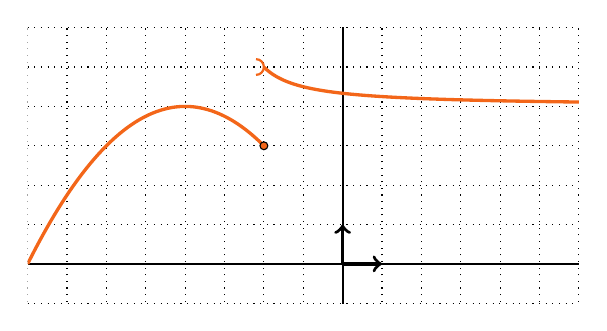
\begin{tikzpicture}[scale=0.5]
\clip (-8,-1) rectangle (6,6);
\draw [thick] (-8,0)--(22,0);
\draw [thick] (0,-4)--(0,28);
\draw [->, very thick] (0,0)--(1,0);
\draw [->,very thick] (0,0)--(0,1);
\draw [ thin, dotted] (-8,-4) grid (22,28);

\draw [very thick, ocre, domain = -2:6, samples =200] plot (\x,{4+1/(\x+3)}) ;
\draw [very thick, ocre, domain = -8:-2, samples =200] plot (\x,{-0.25*\x*\x-2*\x}) ;

\draw [fill=ocre] (-2,3) circle(0.1) ;
\draw [ocre, thick] (-2.2,4.8) arc (-90:90:0.2) ;

\end{tikzpicture}

\end{center}\end{minipage}\hfill\begin{minipage}{0.45\linewidth}


On remarque que 
\begin{itemize}
\item $\displaystyle \lim_{x \to (-2)^-}f(x)=3$ ;
\item $\displaystyle \lim_{x \to (-2)^+}f(x)=5$.\end{itemize}
 Ces deux valeurs sont différentes, la fonction $f$ n'est pas continue en 2. 
 
 Graphiquement, on voit que la courbe de la fonction fait un "saut" en $x=-2$.\end{minipage}\end{example}

\begin{example} On considère la fonction \renewcommand{\arraystretch}{1.2}$f:x\mapsto \left\{ \begin{array}{ll}
2x+9 & \text{si }x<-2\\
x^2+1 & \text{si }-2\leqslant x < 3\\
4x-4 & \text{si } x \geqslant 3
\end{array}\right.$ définie sur $\mathbb{R}$.

\begin{minipage}{0.7\linewidth}
La fonction $f$ est continue sur $]-\infty;-2[$, $]-2;3[$ et $]3;+\infty[$. 

Il faut étudier la continuité aux bords de chaque intervalle.

\paragraph{Continuité en $-2$}
\begin{itemize}
\item $f(-2)=(-2)^2+1=5$ ;
\item  $\displaystyle \lim_{x \to (-2)^-} f(x)=2 \times (-2)+9=5$ ;
\item  $\displaystyle \lim_{x \to (-2)^+} f(x)=(-2)^2+1=5$.
\end{itemize} 

Ainsi, $f$ est continue en $-2$.

\paragraph{Continuité en $3$}
\begin{itemize}
\item $f(3)=4 \times 3 -4 = 8$ ;
\item  $\displaystyle \lim_{x \to 3^-} f(x)=3^2+1=10$.
\end{itemize}

On a $\displaystyle \lim_{x \to 3^-} f(x) \neq f(3)$. Ainsi, $f$ est n'est pas continue en 3.\end{minipage}\hfill\begin{minipage}{0.25\linewidth}


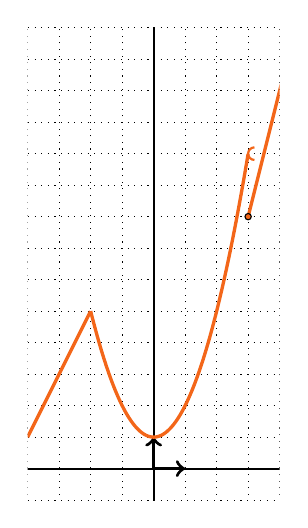
\begin{tikzpicture}[scale=0.4]
\clip (-4,-1) rectangle (4,14);
\draw [thick] (-8,0)--(22,0);
\draw [thick] (0,-4)--(0,28);
\draw [->, very thick] (0,0)--(1,0);
\draw [->,very thick] (0,0)--(0,1);
\draw [ thin, dotted] (-8,-4) grid (22,28);

\draw [very thick, ocre, domain = -4:-2, samples =200] plot (\x,{2*\x+9}) ;
\draw [very thick, ocre, domain = -2:3, samples =200] plot (\x,{\x*\x+1}) ;
\draw [very thick, ocre, domain = 3:6, samples =200] plot (\x,{4*\x-4}) ;

\draw [fill=ocre] (3,8) circle(0.1) ;
\draw [ocre, thick] (3.2,10.2) arc (90:270:0.2) ;

\end{tikzpicture}

\end{minipage}


\end{example}



\begin{proposition} La somme et le produit de fonctions continues sur un intervalle $I$ sont continus sur $I$.\end{proposition}

\begin{example} La fonction $x\mapsto \cos(x)(x^2+3\sqrt{x})-\sin(x)e^x$ est continue sur $\mathbb{R}_+$.\end{example}

\begin{theorem} Soit $f$ une fonction définie sur un intervalle $I$. Si $f$ est dérivable sur $I$, alors $f$ est également continue sur $I$.\end{theorem}

La réciproque est fausse. La fonction $x\mapsto |x|$ est continue sur $\mathbb{R}$ mais n'est pas dérivable en 0.

\begin{minipage}{0.6\linewidth}
Il existe par ailleurs des fonctions continues sur $\mathbb{R}$ qui ne sont dérivables nulle part ! 

Les exemples les plus connus sont sans doute les fonctions de Weierstrass. Ce sont des courbes fractales : peu importe le niveau de zoom que l'on peut avoir sur la courbe, on verra toujours de nouveaux détails apparaître.
\end{minipage}\hfill \begin{minipage}{0.35\linewidth}
\begin{center}
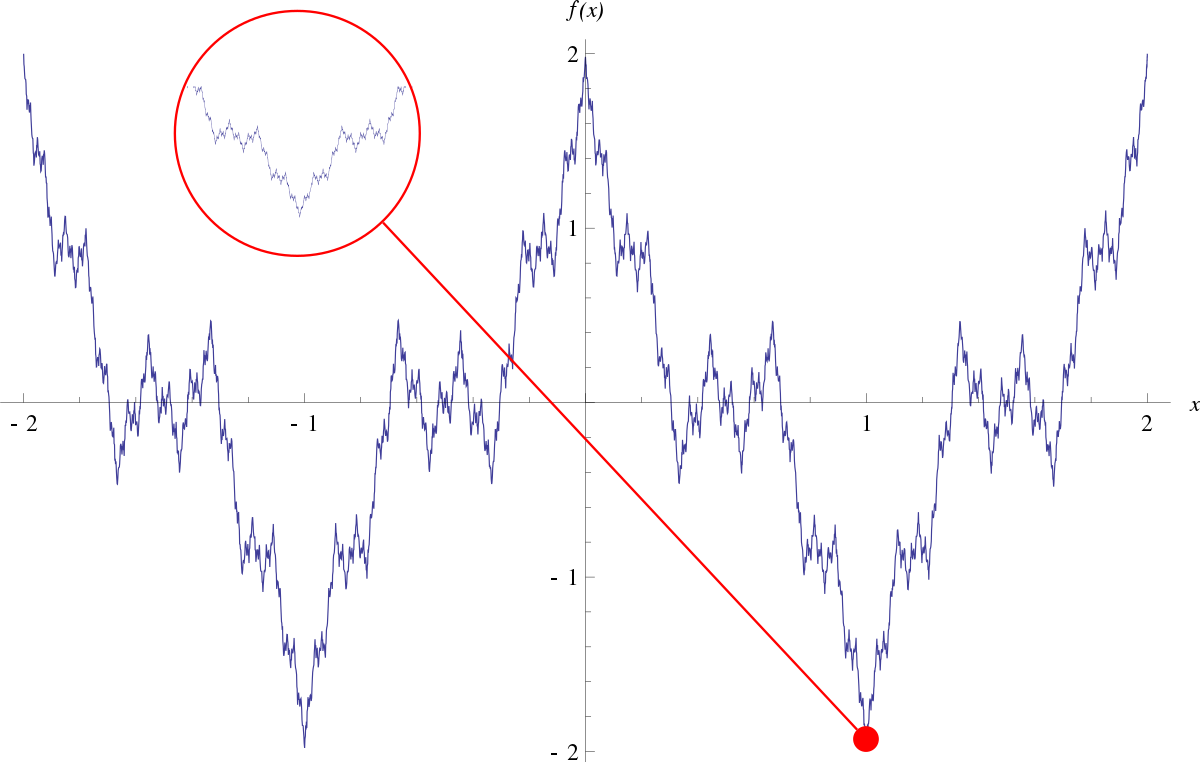
\includegraphics[scale=0.15]{weierstrass}
\end{center}
\end{minipage}



\section{Suites et fonction continue}

\begin{proposition}[Image d'une suite convergente] Soit $I$ un intervalle et $(u_n)$ une suite telle que pour tout entier naturel $n$, $u_n \in I$. Soit $g$ une fonction définie sur l'intervalle $I$. 

Si la suite $(u_n)$ est convergente avec $\displaystyle\lim_{n\to +\infty} u_n=\ell \in I$ et si $g$ est \textbf{continue} en $\ell$, alors $\displaystyle\lim_{n\to +\infty} g(u_n)=g(\ell)$

En d'autres termes, $\displaystyle\lim_{n\to +\infty}g(u_n)=g(\displaystyle\lim_{n\to +\infty} u_n)$.\end{proposition}

\begin{example} Pour tout entier naturel non nul $n$, on note $u_n=\sqrt{9+\dfrac{1}{n}}$.
On a $\displaystyle\lim_{n\to +\infty} \left(9+\dfrac{1}{n}\right)=9$. 

Or, la fonction $x\mapsto \sqrt{x}$ est continue en $9$. Ainsi, $\displaystyle\lim_{n \to+\infty}u_n=\sqrt{9}=3$.
\end{example}

L'hypothèse de continuité est primordiale !
Pour tout réel $x$, notons $\lfloor x \rfloor$ la partie entière du réel $x$, c'est-à-dire le plus grand entier qui soit plus petit que $x$. Par exemple, $\lfloor 1,3 \rfloor = 1$.

Pour tout entier naturel non nul $n$, on note $u_n=1-\dfrac{1}{10^n}$. On a ainsi $u_0=0$, $u_1=0,9$, $u_2=0,999$, $u_3=0,9999$ etc.

\begin{itemize}
\item Pour tout entier naturel non nul, $\lfloor u_n \rfloor = 0$. On a alors $\displaystyle\lim_{n\to +\infty} \lfloor u_n \rfloor = 0$ ;
\item La suite $(u_n)$ est convergente et on a $\displaystyle\lim_{n\to +\infty} u_n = 1$. Ainsi, $\lfloor \displaystyle\lim_{n\to +\infty} u_n \rfloor=\lfloor 1 \rfloor=1$ ;
\item On a donc  $\displaystyle\lim_{n\to +\infty} \lfloor u_n \rfloor \neq \lfloor \displaystyle\lim_{n\to +\infty} u_n \rfloor$. 

On montre en fait que la fonction $x\mapsto  \lfloor x \rfloor$ n'est pas continue en 1.
\end{itemize}

\newpage

\begin{theorem}[Théorème du point fixe]Soit $I$ un intervalle, $g$ une fonction définie et continue sur $I$ et $(u_n)$ une suite telle que pour tout entier naturel $n$, $u_n \in I$ et $u_{n+1}=g(u_n)$.

On suppose que la suite $(u_n)$ est convergente, de limite $\ell\in I$. Alors $g(\ell)=\ell$.\end{theorem}

\begin{demonstration} Pour tout entier naturel $n$, on a $u_{n+1}=g(u_n)$. La suite $(u_n)$ étant convergente, il est possible de passer à la limite dans cette égalité.

Ainsi, $\displaystyle\lim_{n \to +\infty}u_{n+1}=\displaystyle\lim_{n \to +\infty}g(u_n)$. Or, $\displaystyle\lim_{n \to +\infty}u_{n+1}=\ell$ et, la fonction $g$ étant continue sur $I$, on a d'après la propriété précédente que $\displaystyle\lim_{n \to +\infty}g(u_n)=g(\displaystyle\lim_{n \to +\infty}u_n)=g(\ell)$. Ainsi, $g(\ell)=\ell$.
\end{demonstration}

\begin{example}On définit la suite $(u_n)$ par $u_0=2$ et, pour tout entier $n$, $u_{n+1}=\sqrt{3u_n+4}$.

Montrons que la suite $(u_n)$ est croissante et que pour tout entier naturel $n$, $2 \leqslant u_n \leqslant 4$.

Pour tout entier naturel $n$, on considère la proposition $\mathcal{P}(n)$ : « $2\leqslant u_n \leqslant u_{n+1} \leqslant 4$ ».

\begin{itemize}
\item \textbf{Initialisation} : On a $u_0=2$, $u_1=\sqrt{3 \times 2 + 4} =\sqrt{10}$. On a bien $2\leqslant u_0 \leqslant u_{1} \leqslant 4$. $\mathcal{P}(0)$ est donc vraie.
\item \textbf{Hérédité} : Soit $n\in\mathbb{N}$. Supposons que $\mathcal{P}(n)$ est vraie. On a donc $2\leqslant u_n \leqslant u_{n+1} \leqslant 4$.
Or, la fonction $x\mapsto \sqrt{3x+4}$ est croissante sur $[2;4]$. Ainsi, \[\sqrt{3 \times 2+4} \leqslant \sqrt{3 \times u_n +4} \leqslant \sqrt{3 \times u_{n+1} +4} \leqslant \sqrt{3 \times 4 +4},\] c'est-à-dire, \[\sqrt{10} \leqslant u_{n+1} \leqslant u_{n+2} \leqslant 4.\] Puisque $2 \leqslant \sqrt{10}$, on a donc bien \[2\leqslant u_{n+1} \leqslant u_{n+2} \leqslant 4.\] $\mathcal{P}(n+1)$ est donc vraie.
\item \textbf{Conclusion} : Par récurrence $\mathcal{P}(n)$ est vraie pour tout entier naturel $n$.
\end{itemize}

Puisque la suite $(u_n)$ est croissante et majorée, la suite $(u_n)$ converge. Notons $\ell$ sa limite.

Puisque la fonction $g:x\mapsto \sqrt{3x+4}$ est continue sur $\left]-\dfrac{4}{3};+\infty \right[$ et que $l \in [2;4]$, on a alors $g(\ell)=\ell$.

Ainsi, $\sqrt{3\ell+4}=\ell$. En élevant cette inégalité au carré, on a $3\ell+4=\ell^2$, soit $\ell^2-3\ell-4=0$. Il s'agit d'un polynôme du second degré dont les racines sont $-1$ et $4$. Or, il n'est pas possible que la suite tende vers $-1$ puisque celle-ci est supérieure à 2. Ainsi, $\displaystyle\lim_{n \to+\infty}u_n=4$.

\end{example}

\newpage
\section{Théorème des valeurs intermédiaires}

\subsection{Cas général}

\begin{theorem}[Théorème des valeurs intermédiaires] Soit $f$ une fonction \textbf{continue} sur un intervalle $[a;b]$ et $k$ un réel compris entre $f(a)$ et $f(b)$.

Alors \textbf{il existe} (au moins) un réel $c$ dans $[a;b]$ tel que $f(c)=k$.\end{theorem}

\textbf{Illustration :} On représente une fonction $f$ ci-dessous.
\begin{center}

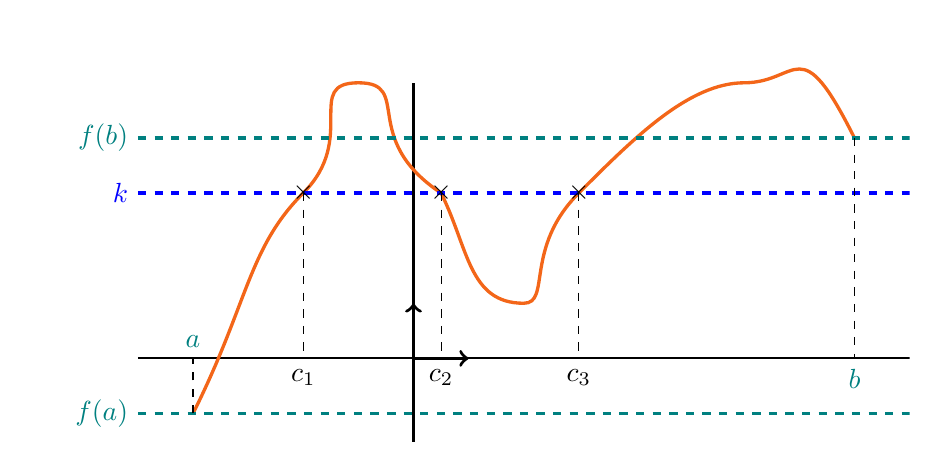
\begin{tikzpicture}[scale=0.7]
\clip (-7,-1.5) rectangle (9,6);
\draw [thick] (-5,0)--(9,0);
\draw [thick] (0,-3)--(0,5);
\draw [->, very thick] (0,0)--(1,0);
\draw [->,very thick] (0,0)--(0,1);

\draw [ocre, very thick] (-4,-1) .. controls (-3,1) and (-3,2) .. (-2,3)
.. controls (-1,4) and (-2,5) .. (-1,5) .. controls (0,5) and (-1,4) ..
(0.5,3) .. controls (1,2) and (1,1) .. (2,1) .. controls (2.5,1) and (2,2) ..
(3,3) .. controls (4,4) and (5,5) .. (6,5) .. controls (7,5) and (7,6) .. (8,4);

\draw [very thick,blue, dashed, domain = -5:9] plot (\x,3);
\draw [very thick,teal, dashed, domain = -5:9] plot (\x,4);
\draw [very thick,teal, dashed, domain = -5:9] plot (\x,-1);

\draw [teal] (-5,4) node[left] {$f(b)$};
\draw [teal] (-5,-1) node[left] {$f(a)$};
\draw [blue] (-5,3) node[left] {$k$};

\draw [very thick] (-2,3) node {$\times$};
\draw [very thick] (0.5,3) node {$\times$};
\draw [very thick] (3,3) node {$\times$};

\draw [dashed] (0.5,3) -- (0.5,0);
\draw [dashed] (-2,3) -- (-2,0);
\draw [dashed] (3,3) -- (3,0);

\draw [dashed] (-4,-1) -- (-4,0);
\draw [dashed] (8,4) -- (8,0);


\draw [very thick] (-2,0) node[below] {$c_1$};
\draw [very thick] (0.5,0) node[below] {$c_2$};
\draw [very thick] (3,0) node[below] {$c_3$};
\draw [teal, very thick] (8,0) node[below] {$b$};
\draw [teal, very thick] (-4,0) node[above] {$a$};

\end{tikzpicture}
\end{center}

Pour tout réel $k$ compris entre $f(a)$ et $f(b)$, $k$ possède au moins un antécédent par $f$. Dans cet exemple, il y en a trois. Le nom de ce théorème se justifie ainsi : une fonction continue qui passe d'une valeur $f(a)$ à une valeur $f(b)$ passe forcément au moins une fois par toutes les valeurs intermédiaires.




\begin{example} On considère la fonction $f:x\mapsto x^3-3x-1$, définie sur $\mathbb{R}$. La fonction $f$ est une fonction polynômiale, elle est donc continue. De plus, $f(-2)=-1$ et $f(2) = 3$.

Or, $0\in[-1;3]$. Ainsi, d'après le théorème des valeurs intermédiaires, il existe (au moins) un réel $c \in[-2;2]$ tel que $f(c)=0$.
\end{example}

Ce théorème ne nous donne aucune indication sur le nombre de ces solutions (en réalité, il y en a 3 sur cet intervalle). Nous verrons dans très peu de temps comment pallier ce problème.

Il est également possible d'utiliser les limites dans le théorème des valeurs intermédiaires.

\begin{theorem}[Théorème des valeurs intermédiaires] Soit $f$ une fonction \textbf{continue} sur un intervalle $]a;b[$ telle que $\displaystyle\lim_{x \to a^+}$ et $\displaystyle\lim_{x\to b^-}f(x)$ existent. Soit $k$ un réel strictement compris entre ces deux limites.

Alors \textbf{il existe} (au moins) un réel $c$ dans $]a;b[$ tel que $f(c)=k$.\end{theorem}


\begin{example}Soit $a$, $b$, $c$ et $d$ quatre réels avec $a> 0$. On considère la fonction $f:x\mapsto ax^3+bx^2+cx+d$, définie sur $\mathbb{R}$.

Pour tout réel non nul, $f(x)=x^3\left(a+\dfrac{b}{x}+\dfrac{c}{x^2}+\dfrac{d}{x^3}\right)$. Or, $\displaystyle\lim_{x\to +\infty}\left(a+\dfrac{b}{x}+\dfrac{c}{x^2}+\dfrac{d}{x^3}\right)=a>0$ et $\displaystyle\lim_{x\to+\infty}x^3=+\infty$. Ainsi, par produit, $\displaystyle\lim_{x\to+\infty}f(x)=+\infty$. De même, on montrer que $\displaystyle\lim_{x\to -\infty}f(x)=-\infty$.

Or, $0\in ]-\infty;+\infty[$. D'après le théorème des valeurs intermédiaires, il existe un réel $x$ tel que $f(x)=0$. Le même raisonnement vaut pour $a<0$ : nous venons de démontrer que tout polynôme de degré 3 admet au moins une racine réelle.\end{example}

\subsection{Fonctions strictement monotones}

\begin{theorem} Soit $f$ une fonction \textbf{continue} et \textbf{strictement monotone} sur un intervalle $[a;b]$ . Soit $k$ un réel strictement compris entre $f(a)$ et $f(b)$ (ou les limites en $a$ et $b$ de $f$). Alors il existe un \textbf{unique} réel $c \in ]a;b[$ tel que $f(c)=k$.\end{theorem}

Là encore, il est possible d'utiliser les limites de $f$ en $a$ et en $b$ si elles existent.

\begin{example} On considère la fonction $f:x\mapsto \dfrac{e^{x-1}}{x}$, définie sur $I=]0;+\infty[$.
Montrons que l'équation $f(x)=2$ possède exactement deux solutions sur l'intervalle $]0;+\infty[$.

D'une part, pour tout $x>0$, $f(x)=\dfrac{e^{x-1}}{x}=\dfrac{1}{e}\times \dfrac{e^x}{x}$. 

Or, par croissances comparées, $\displaystyle\lim_{x \to+\infty}\dfrac{e^x}{x}=+\infty$ et donc $\displaystyle\lim_{x\to+\infty}f(x)=+\infty$. 

Par ailleurs, $\displaystyle\lim_{x\to 0^+}e^{x-1}=e^{-1}>0$ et $\displaystyle\lim_{x \to 0^+}x=0^+$. Par quotient, $\displaystyle\lim_{x \to 0^+}f(x)=+\infty$.

La fonction $f$ est un quotient de fonctions dérivables sur $I$ et son dénominateur ne s'annule pas sur cet intervalle. Ainsi, $f$ est également dérivable sur $I$ et, pour tout réel $x>0$,
\[f'(x)=\dfrac{e^{x-1}\times x - e^{x-1} \times 1}{x^2}=\dfrac{(x-1)e^{x-1}}{x^2}.\]
Or, pour tout réel $x>0$, $e^{x-1}>0$ et $x^2>0$. $f'(x)$ est donc du signe de $x-1$. Ceci nous permet d'établir le tableau de signes de $f'$ et le tableau de variations de $f$.

\begin{center}
  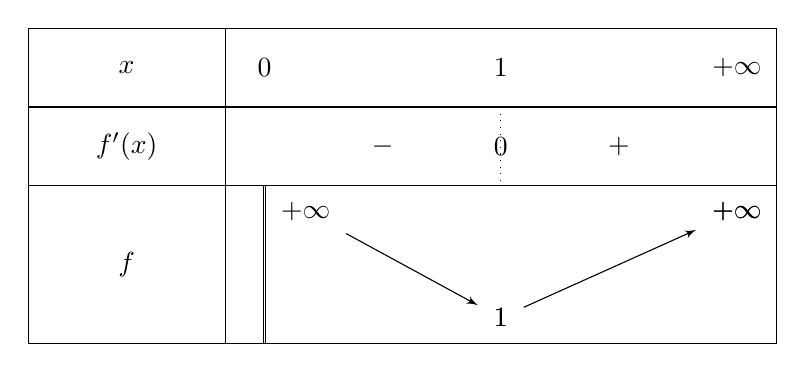
\begin{tikzpicture}[scale=1]
  \tikzset{node style/.style = {inner sep = 2pt, outer sep = 2pt}}
   \tkzTabInit[lgt=2.5]{$x$ / 1 , $f'(x)$ / 1,$f$ / 2}{$0$,$1$,$+\infty$}
	\tkzTabLine{,-,z,+,}
   \tkzTabVar{D+/$+\infty$,-/$1$,+/$+\infty$}     
   \end{tikzpicture}  
 \end{center}
 On raisonne alors selon les intervalles sur lesquels $f$ est strictement monotone.
 
 La fonction $f$ est continue sur $]0;1]$. Or, $\displaystyle\lim_{x\to 0^+}f(x)=+\infty$ et $f(1)=1$. Ainsi, $2 \in ]1 ; +\infty[$. D'après le théorème des valeurs intermédiaires, il existe un réel $c_1\in ]0;1[$ tel que $f(c_1)=2$. De plus, la fonction $f$ est strictement monotone sur l'intervalle $]0;1]$ : la solution à cette équation est donc unique.
 
 De même, il existe un unique réel $c_2\in]1;+\infty[$ tel que $f(c_2)=2$. Finalement, l'équation $f(x)=2$ admet exactement deux solutions sur $]0;+\infty[$.
   


 \end{example}

\newpage

\subsection{Algorithme de dichotomie}

Le théorème des valeurs intermédiaires nous assure de l'existence de solutions à une certaine équation. En revanche, il ne nous indique en rien la valeur de cette solution. Plusieurs algorithmes nous permettent néanmoins d'obtenir au moins une valeur approchée d'une solution de l'équation qui nous intéresse.

Considérons une fonction $f$ continue sur un intervalle $[a;b]$ et $k$ un réel compris entre $f(a)$ et $f(b)$. Dans cet exemple, on supposera par exemple que $f(a) \leqslant k \leqslant f(b)$. Le théorème des valeurs intermédiaires nous assure de l'existence d'un réel $c$ dans l'intervalle $[a;b]$ tel que $f(c)=k$. L'idée, pour obtenir une valeur approchée d'un tel réel, est d'évaluer la valeur prise par la fonction au milieu de l'intervalle $[a;b]$
\begin{itemize}
\item Si $f\left(\dfrac{a+b}{2}\right) < k$, on a alors $f\left(\dfrac{a+b}{2}\right) \leqslant k \leqslant f(b)$. Le théorème des valeurs intermédiaires nous assure alors de l'existence d'une solution à l'équation $f(x)=k$ sur l'intervalle $\left[\dfrac{a+b}{2};b\right]$ ;
\item Si $f\left(\dfrac{a+b}{2}\right) > k$, on a alors $f(a) \leqslant k \leqslant f\left(\dfrac{a+b}{2}\right)$. Le théorème des valeurs intermédiaires nous assure alors de l'existence d'une solution à l'équation $f(x)=k$ sur l'intervalle $\left[a;\dfrac{a+b}{2}\right]$.
\end{itemize}
Dans les deux cas, nous avons trouvé un intervalle deux fois plus petit que l'intervalle $[a;b]$ dans lequel l'équation $f(x)=k$ possède une solution. 

\begin{example}On considère la fonction $f:x\mapsto 3x-e^x$. $f$ est continue, $f(0)=-1$ et $f(1)=3-e>0$. Ainsi, d'après le théorème des valeurs intermédiaires, il existe un réel $c\in[0;1]$ tel que $f(c)=0$.

On calcule alors $f\left(\frac{1}{2}\right)$ : on a $f\left(\frac{1}{2}\right)\simeq -0.15<0$. Ainsi, il existe un réel $c \in \left[ \frac{1}{2} ; 1 \right]$ tel que $f(c)=0$\end{example}

En réitérant le même procédé sur le nouvel intervalle obtenu, on obtiendra alors un intervalle 4 fois plus petit que celui de l'intervalle de départ, puis 8 fois plus petit, 16 fois, 32 fois et ainsi de suite.

On définit en réalité deux suites $(a_n)$ et $(b_n)$ de la manière suivante
\begin{itemize}
\item $a_0=a$ et $b_0=b$ ;
\item Si $f\left(\dfrac{a_n+b_n}{2}\right) < k$, on pose alors $a_{n+1}=\dfrac{a_n+b_n}{2}$ et $b_{n+1}=b_n$ ;
\item Sinon, on pose $a_{n+1}=a_n$ et $b_{n+1}=\dfrac{a_n+b_n}{2}$.
\end{itemize}

Ainsi, pour tout entier naturel $n$, il existe une solution à l'équation $f(x)=0$ dans l'intervalle $[a_n;b_n]$. 

De plus, puisque $b_n-a_n=\dfrac{b-a}{2^n}$, la longueur de l'intervalle $[a_n;b_n]$ tend vers zéro : il est donc possible d'avoir une valeur approchée aussi précise que l'on veut à l'aide de cet algorithme. Cet algorithme peut alors être implémenté en Python

\begin{lstlisting}[language=python]
def dichotomie(a, b, k, f, p) :
	# f est une fonction continue sur [a;b]
	# k est un reel tel que f(a) <= k <= f(b)
	# p designe la precision voulue pour l estimation de la solution
	while b - a >= p :
		m = (a + b) / 2
		if f(m) <= k :
			a = m
		else :
			b = m
	return a
\end{lstlisting}

Dans le cas où $f(a) \geqslant k \geqslant f(b)$, il suffit de changer le sens des inégalités.



\chapter{Exercices}

\section*{Continuité d'une fonction}

\begin{exercise} On considère la fonction \renewcommand{\arraystretch}{1}$f:x\mapsto \left\{ \begin{array}{ll}
6x+8 & \text{si }x\leqslant -1\\
-3x+7 & \text{si }-1< x < 2\\
x-1 & \text{si } x \geqslant 2
\end{array}\right. .$  $f$ est-elle continue en $-1$ ? et en $2$ ?
\end{exercise}

\begin{solution}

\textbf{Continuité en $-1$ ?} :  D'une part, $f(-1)=6\times (-1)+8=2$. D'autre part, $\displaystyle \lim_{x \to (-1)^+} f(x)= -3 \times (-1) +7=10$.

Ainsi, $f$ n'est pas continue en $-1$.

\textbf{Continuité en $2$ ?} : D'une part, $f(2)=2-1=1$. D'autre part, $\displaystyle \lim _{x \to 2^-}=-3\times 2 + 7 = 1$. Enfin, $\displaystyle \lim _{x \to 2^+}=2-1= 1$

La fonction $f$ est continue en $2$.\end{solution}



\begin{exercise}On considère la fonction $f:x\mapsto \left\{ \renewcommand{\arraystretch}{1} \begin{array}{ll}
\frac{1}{2}x -3 & \text{si }x\leqslant -2\\
x+1 & \text{sinon }
\end{array}\right.$ définie sur $\mathbb{R}$.
\vskip10pt
\begin{enumerate}
\item Montrer que la fonction $f$ n'est pas continue en $-2$.
\item Tracer la courbe représentative de la fonction $f$ dans un repère orthonormé.
\end{enumerate}\end{exercise}

\begin{solution}$f(-2)=\dfrac{1}{2}\times(-2)-3=-4$. Or, $\displaystyle\lim_{x \to (-2)^+}=-2+1=-1$. La fonction $f$ n'est pas continue en $-2$.


\begin{center}

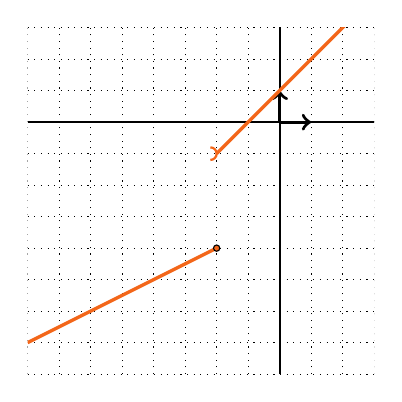
\begin{tikzpicture}[scale=0.4]
\clip (-8,-8) rectangle (3,3);
\draw [thick] (-8,0)--(22,0);
\draw [thick] (0,-8)--(0,28);
\draw [->, very thick] (0,0)--(1,0);
\draw [->,very thick] (0,0)--(0,1);
\draw [ thin, dotted] (-8,-8) grid (22,28);

\draw [very thick, ocre, domain = -8:-2, samples =200] plot (\x,{\x/2-3}) ;
\draw [very thick, ocre, domain = -2:6, samples =200] plot (\x,{\x+1}) ;

\draw [fill=ocre] (-2,-4) circle(0.1) ;
\draw [ocre, thick] (-2.2,-1.2) arc (-90:90:0.2) ;

\end{tikzpicture}

\end{center}
\end{solution}




\begin{exercise}
Soit $a$ et $b$ deux réels. On considère la fonction \renewcommand{\arraystretch}{1}$f:x\mapsto \left\{ \begin{array}{ll} ax^2+bx+1 & \text{si } x<1 \\ x^2+ax+b & \text{si } x\geqslant 1 \end{array}\right.$.\\
Montrer que la fonction $f$ est continue sur $\mathbb{R}$.\end{exercise}
\begin{solution}
 $f$ est continue sur $]-\infty;1[$ et sur $]1;+\infty[$. Il reste à déterminer si elle est continue en $1$.
 \begin{itemize}
 \item $f(1)=1^2+a \times 1+b=1+a+b$ ;
 \item $\displaystyle\lim_{x \to 1^-} f(x)= a \times 1^2 + b \times 1 + 1 = a +b+1$ ;
 \item $\displaystyle\lim_{x \to 1^+} f(x)=1+a+b$.
 \end{itemize}
 Ainsi, $f$ est continue en 1. Finalement, $f$ est continue sur $\mathbb{R}$.\end{solution}
 
 


\begin{exercise}On considère la fonction $f$ définie par $f(0)=0$ et, pour tout réel non nul $x$, $f(x)=\exp\left(-\dfrac{1}{x^2}\right)$. \\ Montrer que $f$ est continue sur $\mathbb{R}$.\end{exercise}

\begin{solution}La fonction $f$ est continue sur $]-\infty ;0[$ et $]0;+\infty[$.

On sait que $\displaystyle\lim_{x\to 0^+}\left(-\dfrac{1}{x^2}\right)=-\infty$. Or, $\displaystyle \lim_{X \to -\infty}e^X=0$. Ainsi, $\displaystyle\lim_{x\to 0^+}f(x)=0$. De la même manière, $\displaystyle\lim_{x\to 0^-}f(x)=0=f(0)$. $f$ est donc continue en 0.\end{solution}

\begin{exercise}
On considère la fonction $f$ définie par $f(0)=0$ et, pour tout réel non nul $x$, $f(x)=x \sin\left(\dfrac{1}{x}\right)$. \\ Montrer que $f$ est continue sur $\mathbb{R}$.\end{exercise}

\begin{solution}La fonction $f$ est continue sur $]-\infty ;0[$ et $]0;+\infty[$.

Pour tout $x>0$, on a $-1 \leqslant \sin\left(\dfrac{1}{x}\right) 1$ et donc $-x \leqslant x\sin\left(\dfrac{1}{x}\right) \leqslant x$. Or, $\displaystyle\lim_{x\to 0^+}(-x)=\displaystyle\lim_{x\to 0^+}x=0$. D'après le théorème d'encadrement, $\displaystyle\lim_{x\to 0^+}f(x)=0$.

De même, on montre que $\displaystyle\lim_{x\to 0^-}f(x)=0$. Ainsi, la fonction $f$ est aussi continue en 0.\end{solution}


\section*{Suites et fonction continue}

\begin{exercise}Déterminer$\displaystyle\lim_{n\to +\infty} \sqrt{\dfrac{4n^2+1}{n^2+3n+2}}$ et $\displaystyle\lim_{n\to +\infty} \exp\left( \dfrac{1}{n}\right)$, en énonçant bien les propriétés utilisées.\end{exercise}


\begin{solution}Pour tout entier naturel non nul $n$, 
\[\dfrac{4n^2+1}{n^2+3n+2}$=$\dfrac{n^2}{n^2} \times \dfrac{4+\frac{1}{n^2}}{1+\frac{3}{n}+\frac{2}{n^2}}=\dfrac{4+\frac{1}{n^2}}{1+\frac{3}{n}+\frac{2}{n^2}}\]
Or, $\displaystyle \lim_{n \to + \infty} \dfrac{4+\frac{1}{n^2}}{1+\frac{3}{n}+\frac{2}{n^2}} = 4$. De plus, la fonction $x\mapsto \sqrt{x}$ est continue en 4. \\ Ainsi, $\displaystyle \lim_{n \to + \infty} \sqrt{\dfrac{4+\frac{1}{n^2}}{1+\frac{3}{n}+\frac{2}{n^2}}}=\sqrt{4}=2$.

On sait que $\displaystyle \lim_{n \to + \infty} \dfrac{1}{n}=0$. De plus, la fonction exponentielle est continue en 0. \\ Ainsi, $\displaystyle \lim_{n \to + \infty}\exp\left(\dfrac{1}{n}\right)=e^0=1$.\end{solution}




\begin{exercise}On considère la fonction $f$ définie par $f(0)=1$ et pour tout réel non nul $x$, $f(x)=\sin\left(\dfrac{1}{x}\right)$. \\ Pour tout entier naturel non nul $n$, on pose $u_n=\dfrac{1}{2n\pi}$.
\begin{enumerate}
\item Que vaut $f(u_n)$ pour tout entier naturel $n$ ?
\item Comparer $\displaystyle\lim_{n \to +\infty}f(u_n)$ et $f(\displaystyle\lim_{n \to + \infty}u_n)$. La fonction $f$ est-elle continue en 0 ?\end{enumerate}\newpage
\end{exercise}


\begin{solution}Pour tout entier naturel $n$, $f(u_n=\sin\left(\dfrac{1}{\frac{1}{2n\pi}}\right)=\sin(2n\pi)=0$.

Ainsi, $\displaystyle\lim_{n \to + \infty}f(u_n)=0$. Or, $\displaystyle\lim_{n\to+\infty}u_n=0$ et $f(0)=1$. Ainsi, $\displaystyle\lim_{n \to +\infty}f(u_n)\neq f(\displaystyle\lim_{n\to+\infty}u_n)$. La fonction $f$ n'est donc pas continue en 0.\end{solution}





\begin{exercise}On considère la suite $(u_n)$ par $u_0=1$ et, pour tout entier naturel $n$, $u_{n+1}=-\dfrac{3}{u_n+1}+3$.
\begin{enumerate}
\item Montrer par récurrence que pour tout entier naturel $n$, $1\leqslant u_n\leqslant 2$ et que la suite $(u_n)$ est croissante.
\item En déduire que la suite $(u_n)$ converge et déterminer la limite de la suite $(u_n)$.
\end{enumerate}\end{exercise}

\begin{solution}Pour tout entier naturel $n$, on note $\mathcal{P}(n)$ la proposition  $1\leqslant u_n\leqslant u_{n+1}\leqslant 2$.
\begin{itemize}
\item $u_0=1$, $u_1=\dfrac{3}{2}$ et on a bien $1\leqslant u_0 \leqslant u_1 \leqslant 2$, $\mathcal{P}(0)$ est donc vraie.
\item Soit $n \in \mathbb{N}$ pour lequel $\mathcal{P}(n)$ est vraie. 

Ainsi, $1 \leqslant u_n \leqslant u_{n+1} \leqslant 2$, d'où $2 \leqslant u_n +1 \leqslant u_{n+1}+1 \leqslant 3$. 

La fonction $x\mapsto \dfrac{1}{x}$ étant décroissante sur $\mathbb{R}_+$, on a alors, $\dfrac{1}{2} \geqslant \dfrac{1}{u_n+1} \geqslant \dfrac{1}{u_{n+1}+1} \geqslant \dfrac{1}{3}$, puis, en multipliant par $-3$ qui est négatif, $\dfrac{-3}{2} \leqslant -\dfrac{3}{u_n+1} \leqslant -\dfrac{3}{u_{n+1}+1} \leqslant -1$ .

Finalement, on a $\dfrac{3}{2} \leqslant u_{n+1} \leqslant u_{n+2} \leqslant 2$. En particulier, puisque $\dfrac{3}{2} >1$, on a $1\leqslant u_{n+1} \leqslant u_{n+2} \leqslant 2$
. \\ $\mathcal{P}(n+1)$ est donc vraie.
\item Ainsi, $\mathcal{P}(0)$ est vraie $P$ est héréditaire. Par récurrence, $\mathcal{P}(n)$ est vraie pour tout $n\in\mathbb{N}$.
\end{itemize}

La suite $(u_n)$ étant croissante et majorée par 2, elle est donc convergente.

La fonction $f:x \mapsto -\dfrac{3}{x+1}+3$ est continue sur $]-1;+\infty [$ et, pour tout entier naturel $n$, on a bien $u_n \in ]-1 ; +\infty [$. Ainsi, la limite $\ell$ de la suite $(u_n)$ vérifie $f(\ell)=\ell$, c'est-à-dire $\ell = -\dfrac{3}{\ell + 1}+3$.

Ainsi, on trouve $\dfrac{\ell(2-\ell)}{\ell+1}=0$ et donc $l=0$ ou $l=2$. Puisque pour tout entier naturel $n$, $u_n \geqslant 1$, le cas $\ell=0$ est impossible. On a donc $\ell=2$.\end{solution}



\begin{exercise}
On considère la suite $(u_n)$ définie par $u_0=0$ et pour tout entier naturel $n$, $u_{n+1}=\sqrt{6+u_n}$.
\begin{enumerate}
\item Supposons que $(u_n)$ converge : quelle peut-être sa limite ?
\item Montrer que pour tout entier naturel $n$, $0\leqslant u_n \leqslant 3$ et que la suite $u_n$ est croissante.
\item Que peut-on en déduire sur la convergence de la suite $(u_n)$ ?
\end{enumerate}
\end{exercise}

\begin{solution}Si $(u_n)$ converge vers un réel $\ell$, puisque la fonction $x\mapsto \sqrt{6+x}$ est continue sur $[-6;+\infty[$, ce réel $\ell$ vérifie $\ell=\sqrt{6+\ell}$. Ainsi, $\ell^2=6+\ell$ ou encore $\ell^2-\ell-6=0$. On trouve alors deux solutions qui sont $\ell=-2$ et $\ell=3$.

Pour tout entier naturel $n$, on note $\mathcal{P}(n)$ la proposition $0\leqslant u_n \leqslant u_{n+1} \leqslant 3$.
\begin{itemize}
\item $u_1= \sqrt{6+0}=\sqrt{6}$. On a bien $0 \leqslant u_0 \leqslant u_1 \leqslant 3$. $\mathcal{P}(0)$ est vraie.
\item Soit $n$ un entier naturel tel que $\mathcal{P(n)}$ soit vraie. Ainsi, $0\leqslant u_n \leqslant u_{n+1} \leqslant 3$. \\ Alors, $6\leqslant 6+u_n \leqslant 6+u_{n+1} \leqslant 9$ . Par ailleurs,  la fonction Racine carrée étant croissante sur $\mathbb{R}_+$, on a $\sqrt{6} \leqslant u_{n+1} \leqslant u_{n+3} \leqslant 3$. Or, puisque $\sqrt{6} \geqslant 0$, on a bien $0\leqslant u_{n+1} \leqslant u_{n+2} \leqslant 3$. $\mathcal{P}(n+1)$ est donc vraie.
\item  $\mathcal{P}(0)$ est vraie et $\mathcal{P}$ est héréditaire. Par récurrence, $\mathcal{P}(n)$ est vraie pour tout $n\in\mathbb{N}$.
\end{itemize}

La suite $(u_n)$ est croissante et majorée, elle est donc convergente. De plus, elle n'a que deux limites possibles qui sont $-2$ et $3$. $-2$ est impossible puisque pour tout entier naturel $n$, $u_n \geqslant 0$. Ainsi, $\displaystyle \lim_{n \to + \infty }u_n=3$.\end{solution}




\begin{exercise}[topic=cont02, subtitle={(Amérique du Nord 2021)}]Un biologiste s'intéresse à l'évolution de la population d'une espèce animale sur une île du Pacifique.

Au début de l'année 2020, cette population comptait 600 individus. On considère que l'espèce sera menacée d'extinction sur cette île si sa population devient inférieure ou égale à 20 individus.

Le biologiste modélise le nombre d'individus par la suite $(u_n)$
définie par par\[\left\{\renewcommand{\arraystretch}{1}\begin{array}{ll}u_0=0,6\\ \text{Pour tout entier naturel }n,\, u_{n+1}=0,75u_n(1-0.15u_n)\end{array}\right.\]
où pour tout entier naturel $n$, $u_n$ désigne le nombre d'individus, en milliers, au début de l'année $2020+n$.
\begin{enumerate}
\item Estimer, selon ce modèle, le nombre d'individus présents sur l'île au début de l'année 2021 puis au début de l'année 2022.
\end{enumerate}
Soit $f$ la fonction définie sur l'intervalle $[0;1]$ par $f(x)=0,75x(1-0.15x)$.
\begin{enumerate}
\setcounter{enumi}{1}
\item  Montrer que la fonction $f$ est croissante sur $[0;1]$ et dresser son tableau de variations.
\item Résoudre dans l'intervalle $[0,1]$ l'équation $f(x)=x$.
\end{enumerate}
On remarquera pour la suite de l'exercice que, pour tout entier naturel $n$, $u_{n+1}=f(u_n)$.
\begin{enumerate}
\setcounter{enumi}{3}
\item \begin{enumerate}
\item Montrer par récurrence que pour tout entier naturel $n$, $0\leqslant u_{n+1} \leqslant u_n \leqslant 1$.
\item En déduire que la suite $(u_n)$ est convergente.
\item Déterminer la limite $l$ de la suite $(u_n)$.
\end{enumerate}
\item Le biologiste a l'intuition que l'espèce sera tôt ou tard menacée d'extinction.
\begin{enumerate}
\item Justifier que, selon ce modèle, le biologiste a raison.
\item Le biologiste a programmé en langage Python la fonction menace() ci-dessous.

\begin{lstlisting}[language=python]
def menace():
	U = 0.6
	N = 0
	while U > 0.02 :
		U = 0.75 * U * (1 - 0.15 * U)
		N = N + 1
	return N
\end{lstlisting}


Donner la valeur numérique renvoyée lorsqu'on appelle la fonction menace().
Interpréter ce résultat dans le contexte de l'exercice.
\end{enumerate}
\end{enumerate}
\newpage
\end{exercise}

\begin{solution}\hspace{0pt}
\begin{enumerate}
\item On a $u_1=0.75 \times 0.6 \times (1-0.75 \times 0.6) = 0.4095$ et $u_2=0.75 \times 0.4095 \times (1-0.75 \times 0.4095) \simeq 0.2882$. Ainsi, il y aura environ 410 individus en 2021 et 288 en 2022.

\item $f$ est dérivable sur $[0;1]$ et pour tout réel $x\in[0;1]$, $f'(x)=0.75 \times(1-0.15x)+0.75x \times (-0.15) = 0.75-0.225x$.\\
Or, si $0 \leqslant x \leqslant 1$, alors $0 \leqslant 0.225x \leqslant 0.225$ d'où $0\geqslant -0.225x \geqslant -0.225$ et $0.75 \geqslant 0.75-0.225x \geqslant 0.525$. En particulier, pour tout $x\in[0;1]$, $f'(x) > 0$ : $f$ est strictement croissante sur $[0;1]$.

\begin{center}
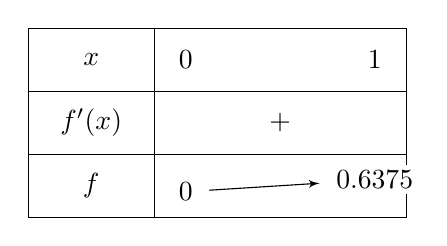
\begin{tikzpicture}[scale=0.8]
   \tkzTabInit{$x$ / 1 , $f'(x)$ / 1, $f$ / 1}{$0$,$1$}
   \tkzTabLine{, +,  }
   \tkzTabVar{-/$0$,+/$0.6375$}
\end{tikzpicture}
\end{center}


\item Soit $x \in [0;1]$. $f(x)=x$ si et seulement si $0.75x(1-0.15x)=x$ soit $0.75x(1-0.15x)-x=0$. En factorisant par $x$, ceci est équivalent à $x(0.75(1-0.15x)-1)=0$, c'est-à-dire $x(-0.25-0.1125x)=0$.

Ainsi, $f(x)=x$ si et seulement si $x=0$ ou $-0.25-0.1125x = 0$, soit $x=0$ ou $x=-\dfrac{0.25}{0.1125}$. Or, $-\dfrac{0.25}{0.1125}<0$. L'unique solution de l'équation $f(x)=x$ sur $[0;1]$ est donc $x=0$.

\item \begin{enumerate}
\item Pour tout entier naturel $n$, on pose $P(n)$ : « $0\leqslant u_{n+1} \leqslant u_n \leqslant 1$ ».
\begin{itemize}
\item On a $u_0=0.6$ et $u_1=0.4095$. On a donc bien $0 \leqslant u_1 \leqslant u_0 \leqslant 1$. $P(1)$ est vraie.
\item Soit $n\in\mathbb{N}$. Supposons $P(n)$ vraie. On a donc $0\leqslant u_{n+1} \leqslant u_n \leqslant 1$. En appliquant la fonction $f$ qui est strictement croissante sur $[0;1]$, on a alors $f(0)\leqslant f(u_{n+1}) \leqslant f(u_n) \leqslant f(1)$, soit $0\leqslant u_{n+2} \leqslant u_{n+1} \leqslant 0.6375$. Puisque $0.6375<1$, on a bien $0\leqslant u_{n+2} \leqslant u_{n+1} \leqslant 1$. $P(n+1)$ est donc vraie.
\item Par récurrence, $P(n)$ est vraie pour tout entier naturel $n$.
\end{itemize}
\item La suite $(u_n)$ est décroissante et minorée, elle est donc convergente vers un réel $\ell$.
\item La fonction $f$ étant continue sur $[0;1]$, on a $f(\ell)=\ell$. Or, l'unique solution de cette équation sur $[0;1]$ est 0. Ainsi, $\displaystyle\lim_{n\to +\infty}u_n=0$.
\end{enumerate}
\item 
\begin{enumerate}
\item D'après les questions précédentes, le nombre d'individus en milliers dans la population étudiée décroît et tend vers 0 : il arrivera donc un moment où cette population sera inférieure à 20 individus.
\item L'algorithme renvoie la valeur 11 : l'espace sera menacée d'extinction en 2031.
\end{enumerate}
\end{enumerate}

\end{solution}






\section*{Théorème des valeurs intermédiaires}


\begin{exercise}Pour tout réel $x>0$, on pose $f(x)=e^x-\dfrac{1}{x}$.
\begin{enumerate}
\item Donner une valeur approchée à $10^{-1 }$ près de $f(1)$ et $f(2)$.
\item En déduire que l'équation $f(x)=2$ possède au moins une solution sur l'intervalle $[1;2]$.\end{enumerate}
\end{exercise}

\begin{solution}On a $f(1)\simeq 1.7$ et $f(2)\simeq 6.9$.

De plus, $f$ est continue sur $[1;2]$. Or, $2 \in [f(1);f(2)]$. Ainsi, d'après le théorème des valeurs intermédiaires, l'équation $f(x)=2$ possède au moins une solution sur l'intervalle $[1;2]$.\end{solution}




\begin{exercise}[topic=cont03, subtitle={(Amérique du Nord 2023)}]
On considère une fonction $h$ continue sur l'intervalle $[-2;4]$ telle que $h(-1)=0$, $h(1)=4$ et $h(3)=-1$. Parmi les affirmations suivantes, quelle est l'unique affirmation correcte ?
\begin {itemize}
\item La fonction $h$ est croissante sur $[-1;1]$ ;
\item la fonction $h$ est positive sur l'intervalle $[-1;1]$ ;
\item il existe au moins un nombre réel $\alpha$ dans l'intervalle $[1;2]$ tel que $h(\alpha)=1$ ;
\item l'équation $h(x)=1$ admet exactement deux solutions sur l'intervalle $[-2;4]$.
\end{itemize}
\end{exercise}

\begin{solution}L'affirmation correcte est l'affirmation 3 : il s'agit d'une simple application du théorème des valeurs intermédiaires.

Les images de -1 et de 1 par $h$ ne nous donnent aucune information sur le comportement de $h$ entre $-1$ et $1$ : on pourrait très bien avoir $h(0)=-5$ par exemple, ce qui contredirait les affirmations 1 et 2. L'affirmation 4 est fausse : on pourrait avoir $h(0)=h(2)=h(4)=1$. En revanche, si la fonction $h$ était strictement monotone sur les intervalles $[-1;1]$ et $[1;3]$, on aurait alors en effet exactement deux solutions à l'équation $h(x)=1$.\end{solution}




\begin{exercise}
On considère la fonction $f:x \mapsto e^x+x$, définie sur $\mathbb{R}$.
\begin{enumerate}
\item Justifier que $f$ est continue et dérivable sur $\mathbb{R}$ et déterminer $f'(x)$ pour tout réel $x$.
\item Quel est le sens de variation de $f$ sur l'intervalle $[-1;0]$ ?
\item Que vaut $f(0)$ ? Quel est le signe de $f(-1)$ ?
\item En déduire que l'équation $e^x+x=0$ admet exactement une solution sur $[-1;1]$.
\end{enumerate}\end{exercise}

\begin{solution}
 $f$ est dérivable comme somme de fonctions dérivables (et est donc continue). Pour tout réel $x$, $f'(x)=e^x+1$. Puisque pour tout réel $x$, $e^x>0$, il en vient que $f'$ est strictement positive sur $\mathbb{R}$ (et en particulier sur $[-1;0]$). La fonction $f$ est donc strictement croissante sur $[-1;2]$. Par ailleurs, $f(0)=1$ et $f(-1)=e^{-1}-1<0$.
 
Reprenons les informations des questions précédentes :
La fonction $f$ est continue sur $[-1;0]$. On a $f(-1)<0$ et $f(0)>0$. Ainsi, d'après le théorème des valeurs intermédiaires, l'équation $f(x)=0$ admet au moins une solution sur $[-1;0]$. De plus, la fonction $f$ étant strictement croissante sur cet intervalle, une telle solution est unique.\end{solution}




\begin{exercise} On considère la fonction $f:x \mapsto 2x^3+9x^2-60x+3$, définie sur $\mathbb{R}$.
\begin{enumerate}
\item Étudier les variations de la fonction $f$.
\item En déduire la nombre de solutions de l'équation $f(x)=0$ sur $\mathbb{R}$.
\end{enumerate}\end{exercise}

\begin{solution}La fonction $f$ est dérivable sur $\mathbb{R}$. Pour tout réel $x$,  $f'(x)=6x^2+18x-60=6(x^2+3x-10)$. Ainsi, $f'(x)=0 \Leftrightarrow x=2 \text{ ou } x=-5$. On a par ailleurs $f(2)=-65$ et $f(-5)=278$. En outre, $\displaystyle\lim_{x \to +\infty} f(x)=+\infty$ et $\displaystyle \lim_{x \to -\infty} f(x)=-\infty$. Le tableau de variations de $f$ est le suivant.

\begin{center}
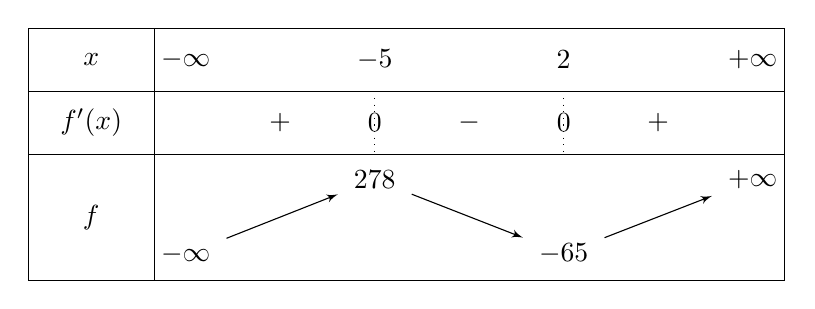
\begin{tikzpicture}[scale=0.8]
   \tkzTabInit{$x$ / 1 , $f'(x)$ / 1, $f$ / 2}{$-\infty$, $-5$,$2$, $+\infty$}
   \tkzTabLine{, +, z,-,z, +,  }
   \tkzTabVar{-/$-\infty$,+/$278$,-/$-65$,+/$+\infty$}
\end{tikzpicture}
\end{center}

On peut en déduire le nombre de solutions de l'équation $f(x)=0$. Par exemple, sur $]-\infty ;-5[$ :
\begin{itemize}
\item La fonction $f$ est continue et strictement monotone ;
\item $f(-5)>0$ et $\displaystyle\lim_{x \to -\infty} f(x)=-\infty$ ;
\item Ainsi, d'après le théorème des valeurs intermédiaires pour les fonctions strictement monotones, l'équation $f(x)=0$ possède une unique solution sur l'intervalle $]-\infty ; -5[$.
\end{itemize}
De la même manière, l'équation $f(x)=0$ admet une unique solution sur $]-5;2[$ puis une unique solution sur $]2;+\infty[$. Ainsi, l'équation $f(x)=0$ possède exactement 3 solutions sur $\mathbb{R}$.\end{solution}




\begin{exercise}Montrer que l'équation $x^3-5x^2+3x+1=0$ admet exactement trois solutions réelles.\end{exercise}

\begin{solution} $f$ est dérivable (et donc continue) sur $\mathbb{R}$. De plus, pour tout réel $x$, $f'(x)=3x^2-10x+3=3(x-3)\left(x-\dfrac{1}{3}\right)$. Les racines peuvent aussi se calculer à l'aide de la méthode du discriminant. On peut alors dresser le tableau de variations de $f$.

\begin{center}
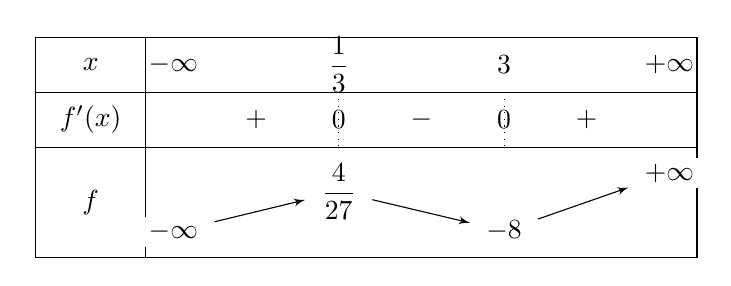
\begin{tikzpicture}[scale=0.7]
   \tkzTabInit{$x$ / 1 , $f'(x)$ / 1, $f$ / 2}{$-\infty$, $\dfrac{1}{3}$ ,$3$ ,$+\infty$}
   \tkzTabLine{, +, z, -,z,+,  }
   \tkzTabVar{-/$-\infty$,+/$\dfrac{4}{27}$,-/$-8$,+/$+\infty$}
\end{tikzpicture}
\end{center}

En appliquant le théorème des valeurs intermédiaires pour les fonctions strictement monotones sur chacun des intervalles $\left]-\infty ; \dfrac{1}{3}\right ]$, $\left[ \dfrac{1}{3}; 3 \right]$ et $[3;+\infty [$, on en déduit que l'équation $f(x)=0$ possède exactement 3 solutions.\end{solution}




\begin{exercise}[topic=cont03, subtitle={(Métropole 2021)}]

On considère la fonction $f$ définie pour tout réel $x\in ]0;+\infty[$ par $f(x)=\dfrac{e^x}{x}$. 
\begin{enumerate}
\item Justifier que $f$ est dérivable sur $]0;+\infty[$ et donner une expression de sa dérivée.
\item Construire le tableau de variations de $f$ sur $]0;+\infty[$. On précisera les limites en $0$ et en $+\infty$.
\item Soit $m\in\mathbb{R}$. Déterminer le nombre de solutions de l'équation $f(x)=m$ en fonction de la valeur de $m$.
\end{enumerate}
\end{exercise}

\begin{solution}$f$ est dérivable comme quotient de fonctions dérivables sur $]0;+\infty[$ et dont le dénominateur ne s'annule pas sur cet intervalle. Pour tout réel $x>0$, $f'(x)=\dfrac{e^x \times x - e^x \times 1}{x^2}=\dfrac{(x-1)e^x}{x^2}$.

Puisque pour tout $x>0$, $e^x>0$ et $x^2>0$, $f'(x)$ est du signe de $x-1$. Par ailleurs, par croissances comparées, $\displaystyle\lim_{x\to +\infty}f(x)=+\infty$. Enfin, par opérations sur les limites, $\displaystyle\lim_{x\to 0^+}f(x)=+\infty$.

\begin{center}
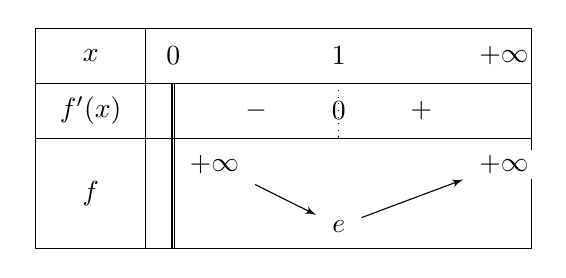
\begin{tikzpicture}[scale=0.7]
   \tkzTabInit{$x$ / 1 , $f'(x)$ / 1, $f$ / 2}{$0$, $1$,  $+\infty$}
   \tkzTabLine{d, -, z, +,  }
   \tkzTabVar{D+/$+\infty$,-/$e$,+/$+\infty$}
\end{tikzpicture}
\end{center}


Ainsi,
\begin{itemize}
\item si $m<e$, l'équation $f(x)=m$ ne possède aucune solution sur $]0;+\infty[$.
\item si $m=e$, l'équation $f(x)=m$ possède une unique solution sur $]0;+\infty[$ : il s'agit de $x=1$.
\item si $m>e$, l'équation $f(x)=m$ possède deux solutions sur $]0;+\infty[$ : l'une sur l'intervalle $]0;1[$, l'autre sur l'intervalle $]1;+\infty[$.
\end{itemize}
\end{solution}




\begin{exercise}[topic=cont03, subtitle={(Centres étrangers 2023)}]
Un biologiste a modélisé l'évolution d'une population de bactéries (en milliers d'entités) par la fonction $f$ définie sur $[0;+\infty[$ par $f(t)=e^3-e^{-0.5t^2+t+2}$. où $t$ désigne le temps en heures depuis le début de l'expérience.

À partir de cette modélisation, il propose les trois affirmations ci-dessous. Pour chacune d'elles, indiquer, en justifiant, si elle est vraie ou fausse.
\begin{itemize}
\item \textbf{Affirmation 1} : « La population augmente en permanence ».
\item \textbf{Affirmation 2} : « À très long terme, la population dépassera 21 000 bactéries ».
\item \textbf{Affirmation 3} : « La population de bactéries aura un effectif de 10 000 à deux reprises au cours du temps ».\end{itemize}
\end{exercise}

\begin{solution}\hspace{0pt}

\begin{itemize}
\item  \textbf{Faux} : $f$ est dérivable sur $[0;+\infty[$ et, pour tout réel $t>0$, \[f'(t)=-(-t+1)e^{-0.5t^2+t+2}=(t-1)e^{-0.5t^2+t+2}\] $f'(t)$ est du signe de $t-1$. On peut alors construire le tableau de variations de $f$.

\begin{center}
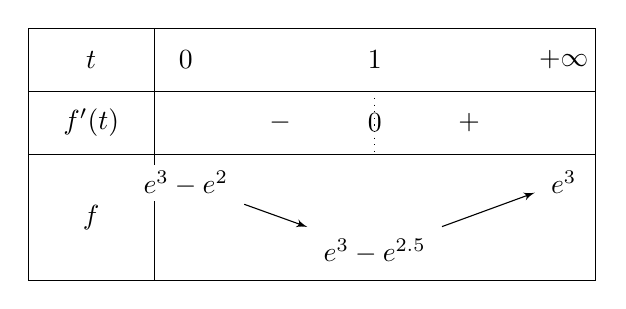
\begin{tikzpicture}[scale=0.8]
   \tkzTabInit{$t$ / 1 , $f'(t)$ / 1, $f$ / 2}{$0$, $1$,  $+\infty$}
   \tkzTabLine{, -, z, +,  }
   \tkzTabVar{+/$e^3-e^2$,-/$e^3-e^{2.5}$,+/$e^3$}
\end{tikzpicture}
\end{center}

En particulier, $f(1)<f(0)$. La population ne fait pas qu'augmenter en permanence.
\item \textbf{Faux :}  On a $\displaystyle\lim_{t\to+\infty}f(t)=e^3 \simeq 20.08$. Par ailleurs, la fonction $f$ est croissante sur $[1;+\infty[$. Ainsi, pour tout $t>1$, $f(t)\leqslant 20.08$. En particulier, la population ne dépasse 21000 bactéries.

\item \textbf{Vrai : } La fonction $f$ est continue sur $[0;1]$. Par ailleurs, $f(0)=e^3-e^2 >10$ et $f(1)=e^3-e^{2.5}<10$. D'après le théorème des valeurs intermédiaires, il existe un réel $t\in ]0;1[$ tel que $f(t)=10$. La fonction $f$ étant strictement décroissante sur cet intervalle, une telle solution est unique. De même, il existe un unique réel $t_2 \in [1;+\infty[$ tel que $f(t_2)=10$. Finalement, 10 possède exactement deux antécédents par la fonction $f$ : la population de bactéries aura donc un effectif de 10000 à deux reprises.\end{itemize}

\end{solution}




\begin{exercise}On considère la fonction $f$ définie pour tout réel $x$ par $f(x)=x^5-3x^4+2x+1$. On note $\mathcal{C}_f$ la courbe représentative de $f$ dans un repère orthonormé.
\begin{enumerate}
\item Déterminer l'équation réduite de $\mathcal{T}$, la tangente à $\mathcal{C}_f$ à l'abscisse 1.
\item Montrer qu'il existe une unique autre tangente à $\mathcal{C}_f$ qui soit parallèle à $\mathcal{T}$. 
\end{enumerate}
\end{exercise}

\begin{solution}Pour tout réel $x$, $f'(x)=5x^4-12x^3+2$. Ainsi, $f'(1)=-5$. Par ailleurs, $f(1)=1$. Ainsi, l'équation réduite de $\mathcal{T}$ est $y=-5(x-1)+1$ soit $y=-5x+6$.

La deuxième question revient à montrer que l'équation $f'(x)=-5$ possède exactement deux solutions sur $\mathbb{R}$ (l'une de ces solutions étant $x=1$). Pour tout réel $x$, $f''(x)=20x^3-36x^2=x^2(20x-36)$. Ainsi, pour tout réel $x$, $f''(x)$ est du signe de $20x-36$. Par ailleurs, par opérations sur les limites $\displaystyle\lim_{x \to -\infty}f(x)=+\infty$. 

Enfin, pour tout réel $x>0$, $f'(x)=x^4\left(5-\dfrac{12}{x}+\dfrac{2}{x^4}\right)$ et donc$\displaystyle\lim_{x \to +\infty}f(x)=+\infty$. Ceci nous permet de dresser le tableau de variations de $f'$.

\begin{center}
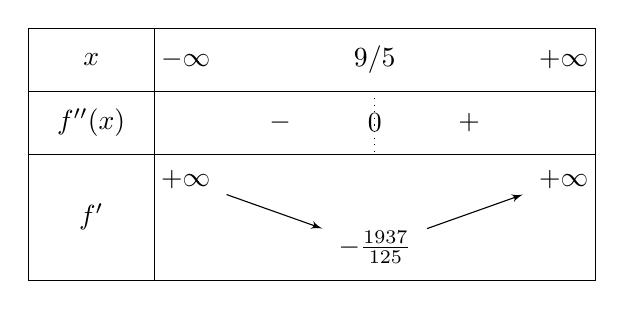
\begin{tikzpicture}[scale=0.8]
   \tkzTabInit{$x$ / 1 , $f''(x)$ / 1, $f'$ / 2}{$-\infty$, $9/5$,  $+\infty$}
   \tkzTabLine{, -,z,+,  }
   \tkzTabVar{+/$+\infty$,-/$-\frac{1937}{125}$,+/$+\infty$}
\end{tikzpicture}
\end{center}

Or, $f'$ est continue sur $\left[ \dfrac{9}{5} ; +\infty\right[$. Par ailleurs, $-5 \in \left[ f\left(\dfrac{9}{5}\right) ; +\infty\right[$. D'après le théorème des valeurs intermédiaires, l'équation $f'(x)=-5$ possède une unique solution sur l'intervalle $\left[ \dfrac{9}{5} ; +\infty \right[$. Si l'on note $\alpha$ cette solution, ceci signifie que la tangente à $\mathcal{C}_f$ à l'abscisse $\alpha$ est parallèle à $\mathcal{T}$. L'équation $f'(x)=-5$ admet également une unique solution sur $\left] - \infty; \dfrac{9}{5} \right]$, mais cette solution n'est autre que $x=1$.

\end{solution}





\begin{exercise}Pour tout réel $x$, on pose $f(x)=x^5-2x-4$. 
\begin{enumerate}
\item Calculer $f(1)$ et $f(2)$.
\item En déduire que l'équation $x^5-2x-4=0$ possède au moins une solution sur $[1;2]$.
\item Écrire les 3 premières étapes de l'algorithme de dichotomie et donner un intervalle de longueur $\frac{1}{8}$ qui contient une solution de l'équation $x^5-2x-4=0$.
\item Donner une solution de cette équation au centième près.\end{enumerate}\end{exercise}

\begin{solution}
On a $f(1)=-5<0$ et $f(2)=24>0$. La fonction $f$ étant continue, d'après le théorème des valeurs intermédiaires, il existe un réel $c \in [1;2]$ tel que $f(c)=0$.

\begin{itemize}
\item Calculons alors $f(1.5)$ : On a $f(1.5)\simeq 0.59$. Ainsi, il existe un réel $c \in [1 ;1.5]$ tel que $f(c)=0$.
\item Calculons alors $f(1.25)$ : On a $f(1.25)\simeq -3.45<0$. Ainsi, il existe un réel $c \in [1.25 ;1.5]$ tel que $f(c)=0$.
\item Calculons alors $f(1.375)$ : On a $f(1.375)\simeq -1.84<0$. Ainsi, il existe un réel $c \in [1.375 ;1.5]$ tel que $f(c)=0$.
\end{itemize}
En poursuivant ainsi, on trouve que $c\simeq 1.47$
\end{solution}



\begin{exercise}Soit $f$ et $g$ les fonction définies pour tout réel $x$ par $f(x)=(1-x)e^x+1$ et $g(x)=\dfrac{x}{e^x+1}$.
\begin{enumerate}
\item Construire le tableau de variations de $f$ en y incluant les limites.
\item En déduire que l'équation $f(x)=0$ admet une unique solution sur $\mathbb{R}$ et en donner une valeur à $10^{-2}$ près. On note $\alpha$ ce réel.
\item Montrer que pour tout réel $x$, $g'(x)=\dfrac{f(x)}{(1+e^x)^2}$.
\item Construire le tableau de variations de $g$.
\end{enumerate}\end{exercise}

\begin{solution}\hspace{0pt}
\begin{enumerate}
\item On a $\displaystyle\lim_{x \to + \infty}(1-x)=-\infty$ et $\displaystyle\lim_{x \to +\infty}e^x=+\infty$. Par produit, $\displaystyle\lim_{x \to + \infty}(1-x)e^x=-\infty$ et donc $\displaystyle\lim_{x \to + \infty}f(x)=-\infty$.

Par ailleurs, pour tout réel $x$, $f(x)=e^x-xe^x+1$. Or, $\displaystyle\lim_{x \to - \infty}e^x=0$ et, par croissances comparées, $\displaystyle\lim_{x \to - \infty}xe^x=0$. Ainsi, $\displaystyle\lim_{x \to - \infty}=1$.

$f$ est par ailleurs dérivable sur $\mathbb{R}$ et pour tout réel $x$, $f'(x)=(-1) \times e^x + (1-x)e^x = -xe^x$, qui est donc du signe de $-x$.

\begin{center}
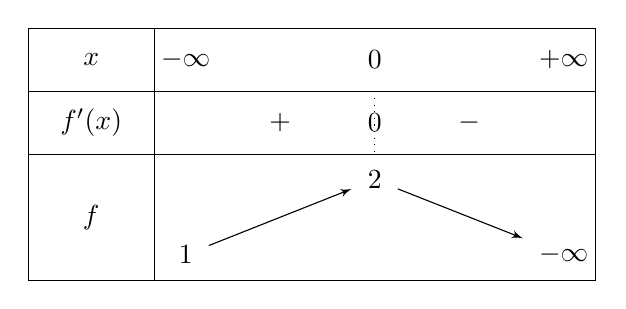
\begin{tikzpicture}[scale=0.8]
   \tkzTabInit{$x$ / 1 , $f'(x)$ / 1, $f$ / 2}{$-\infty$, $0$,  $+\infty$}
   \tkzTabLine{, +,z,-,  }
   \tkzTabVar{-/$1$,+/$2$,-/$-\infty$}
\end{tikzpicture}
\end{center}

\item Pour tout réel $x<0$, $f'(x)>1$ et en particulier, $f'(x)>0$. Par ailleurs, $f$ est continue sur $[0;+\infty[$ et $ 0 \in ]-\infty;2]$. Ainsi, d'après le théorème des valeurs intermédiaires, il existe un réel $\alpha >0$ tel que $f(\alpha)=0$. De plus, la fonction $f$ étant strictement décroissante sur $[0;+\infty[$, un tel réel est unique. En utilisant la calculatrice, on trouve $x\simeq 1.28$.

\item Pour tout réel $x$, $g'(x)=\dfrac{1 \times (e^x+1)-x \times e^x}{(e^x+1)^2}=\dfrac{(1-x)e^x+1}{(e^x+1)^2}=\dfrac{f(x)}{(1+e^x)^2}$.

\item Puisque pour tout réel $x$, $(1+e^x)^2>0$, $g'(x)$ est du signe de $f$.


\begin{center}
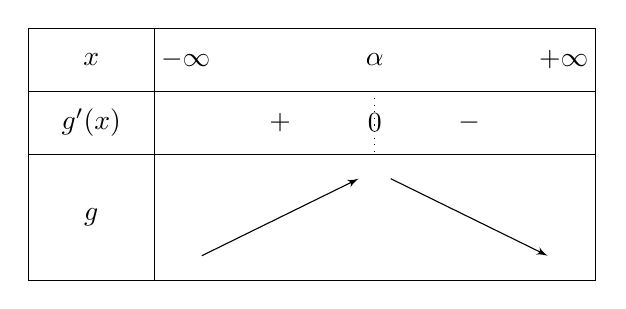
\begin{tikzpicture}[scale=0.8]
   \tkzTabInit{$x$ / 1 , $g'(x)$ / 1, $g$ / 2}{$-\infty$, $\alpha$,  $+\infty$}
   \tkzTabLine{, +,z,-,  }
   \tkzTabVar{-/$ $,+/$ $,-/$ $}
\end{tikzpicture}
\end{center}
\end{enumerate}
\end{solution}



\begin{exercise}[topic=cont03, subtitle={(Centres étrangers 2023)}]

Soit deux réels $a$ et $b$ avec $a<b$. On considère une fonction $f$ définie, continue, strictement croissante sur l'intervalle $[a;b]$ et qui s'annule en un réel $\alpha$. Parmi les propositions suivantes, quelle est la fonction en langage Python qui permet de donner une valeur approchée de $\alpha$ à 0.001 près ?

\begin{minipage}{0.23\linewidth}
\begin{lstlisting}[language=python]
#Algorithme A

def racine(a,b) :
	while abs(b-a) >= 0.001 :
		m = (a+b)/2
		if f(m) < 0 :
			b = m
		else :
			a = m
		return m
\end{lstlisting}
\end{minipage}\hfill\begin{minipage}{0.23\linewidth}
\begin{lstlisting}[language=python]
#Algorithme B

def racine(a,b) :
	m = (a+b) / 2
	while abs(b-a) >= 0.001 :
		if f(m) < 0 :
			a = m
		else :
			b = m
		return m
\end{lstlisting}
\end{minipage}\hfill\begin{minipage}{0.23\linewidth}
\begin{lstlisting}[language=python]
#Algorithme C

def racine(a,b) :
	m = (a+b)/2
	while abs(b-a) <= 0.001 :
		if f(m) < 0 :
			a = m
		else :
			b = m
		return m
\end{lstlisting}
\end{minipage}\hfill\begin{minipage}{0.23\linewidth}
\begin{lstlisting}[language=python]
#Algorithme D

def racine(a,b) :
	while abs(b-a) >= 0.001 :
		m = (a+b)/2
		if f(m) < 0 :
			a = m
		else :
			b = m
		return m
\end{lstlisting}
\end{minipage}\end{exercise}

\begin{solution}Puisque $f$ est strictement croissante sur $[a,b]$, on en déduit que $f(a)<0$ et que $f(b)>0$.

Dans les algorithmes B et C, la valeur de $m$ n'est pas mise à jour à l'intérieur de la boucle while. Ils ne peuvent donc pas être les bons algorithmes. 

Si $f(m)<0$, cela signifie que $f(a)$ et $f(m)$ sont du même signe, il faut donc remplacer la valeur de $a$ par celle de $m$. Le bon algorithme est l'algorithme D.\end{solution}





\begin{exercise}Soit $f$ une fonction continue sur $[0,1]$ telle que, pour tout réel $x \in[0;1]$, on a $f(x) \in[ 0;1]$. Montrer que l'équation $f(x)=x$ admet au moins une solution sur $[0;1]$.\newpage
\end{exercise}

\begin{solution}Pour tout réel $x$, on pose $g(x)=f(x)-x$. $g$ est continue sur $[0;1]$. De plus, $g(0)=f(0)-0\geqslant 0$ et $g(1)=f(1)-1\leqslant 0$ puisque $f(1)\in [0;1]$. D'après le théorème des valeurs intermédiaires, il existe un réel $c \in [0;1]$ tel que $g(c)=0$, c'est-à-dire $f(c)-c=0$ ou encore $f(c)=c$.\end{solution}


\begin{exercise}[subtitle={(Démontrer le théorème des valeurs intermédiaires)}]

Le but de cet exercice est de démontrer le théorème des valeurs intermédiaires... Mais pour commencer, nous avons besoin de résultats supplémentaires sur les suites.

\paragraph{Partie A}

Soit $(a_n)$ et $(b_n)$ deux suites réelles. On dit que $(a_n)$ et $(b_n)$ sont adjacentes si
\begin{itemize}
\item $(a_n)$ est croissante et $(b_n)$ est décroissante ;
\item $\displaystyle \lim_{n \to + \infty} (a_n-b_n)=0$.
\end{itemize}
L'objectif de cette première partie est de démontrer que deux suites adjacentes sont convergentes et de même limite.

\begin{enumerate}
\item Pour tout entier naturel $n$, on pose $c_n = b_n-a_n$.
\begin{enumerate}
\item Montrer que la suite $(c_n)$ est décroissante.
\item Montrer que pour tout entier naturel $n$, $c_n \geqslant 0$ et en déduire que $a_n \leqslant b_n$.
\end{enumerate}
\item Justifier que, pour tout entier naturel $n$, $a_n \leqslant b_0$ et $b_n \geqslant a_0$. \\ Que peut-on en déduire sur les suites $(a_n)$ et $(b_n)$ ?
\item Montrer que $(a_n)$ et $(b_n)$ ont même limite.
\end{enumerate}

\paragraph{Partie B}

Soit $f$ une fonction continue sur un intervalle $[a,b]$, avec $a<b$. Soit $k$ un réel compris entre $f(a)$ et $f(b)$. On suppose que $f(a) < k < f(b)$. On considère alors les suites $(a_n)$ et $(b_n)$ définies par

\begin{itemize}
\item $ a_0 = a 
\text{ et, pour tout entier naturel }n,\, a_{n+1} = \left\{ \begin{array}{ll} a_n& \text{ si } f\left(\dfrac{a_n+b_n}{2}\right) \geqslant k \\ \dfrac{a_n +b_n}{2} &\text{ si } f\left(\dfrac{a_n+b_n}{2}\right) < k \end{array}\right.$
\vskip5pt
\item $ b_0 = b
\text{ et, pour tout entier naturel }n,\, b_{n+1} = \left\{ \begin{array}{ll} \dfrac{a_n +b_n}{2} & \text{ si } f\left(\dfrac{a_n+b_n}{2}\right) \geqslant k \\
b_n &\text{ si } f\left(\dfrac{a_n+b_n}{2}\right) < k \\  \end{array}\right.$
\end{itemize}

Le but est évidemment de montrer que ces suites sont adjacentes. Dans l'ensemble des questions suivantes, il faudra raisonner par disjonction de cas, suivant la valeur de $f\left(\dfrac{a_n+b_n}{2}\right)$.

\begin{enumerate}
\item Montrer par récurrence que, pour tout entier naturel $n$, $a_n \leqslant b_n$. 
\item Montrer que la suite $(a_n)$ est croissante et que la suite $(b_n)$ est décroissante.
\item Montrer que pour tout entier naturel $n$, $b_{n+1}-a_{n+1}=\dfrac{b_n-a_n}{2}$.
\item En déduire $\displaystyle\lim_{n \to + \infty}(b_n-a_n)$. Que peut-on en conclure sur les suites $(a_n)$ et $(b_n)$ ?
\item Montrer que pour tout entier naturel $n$, $f(a_n) \leqslant k \leqslant f(b_n)$.
\item On note $\ell$ la limite commune de $(a_n)$ et $(b_n)$ et on rappelle que $f$ est continue sur $[a,b]$.\\ Montrer que $f(\ell)=k$.
\end{enumerate}

\end{exercise}


\begin{solution}
\textbf{Partie A}

\begin{enumerate}
\item \begin{enumerate}
\item Pour tout entier naturel $n$, $c_{n+1}-c_n = b_{n+1}-a_{n+1}-(b_n-a_n)=b_{n+1}-b_n-(a_{n+1}-a_n)$.
Or, $(b_n)$ est décroissante et donc $b_{n+1}-b_n \leqslant 0$. $(a_n)$ est croissante et donc $-(a_{n+1}-a_n) \leqslant 0$. \\Ainsi, $c_{n+1}-c_n \leqslant 0$. La suite $(c_n)$ est décroissante.
\item La suite $(c_n)$ est décroissante et de limite 0. Ainsi, pour tout $n\in \mathbb{N}$, $c_n \geqslant 0$ et donc $a_n \leqslant b_n$.
\end{enumerate}
\item Pour tout entier naturel $n$, $a_n \leqslant b_n$. Or, $(b_n)$ est décroissante et donc, pour tout entier naturel $n$, $b_n \leqslant b_0$. Ainsi, pour tout entier naturel $n$, $a_n \leqslant b_0$. Un raisonnement similaire permet de conclure que, pour tout entier naturel $n$, $b_n \geqslant a_0$. La suite $(a_n)$ est donc croissante et majorée par $b_0$, la suite $(b_n)$ est décroissante et minorée par $a_0$. Ces deux suites sont donc convergentes.
\item Notons $l_1$ la limite de $(a_n)$ et $l_2$ la limite de $(b_n)$. On sait que $\displaystyle\lim_{n \to + \infty}(a_n-b_n)=0$. \\
Or, $\displaystyle\lim_{n \to + \infty}(a_n-b_n)=\displaystyle\lim_{n \to + \infty}a_n-\displaystyle\lim_{n \to + \infty}b_n=l_1-l_2$. Ainsi, $l_1-l_2=0$ et donc $l_1=l_2$.
\end{enumerate}

\textbf{Partie B}


\begin{enumerate}
\item Pour tout entier naturel $n$, on pose $P(n)$ : « $a_n \leqslant b_n$ » . 
\begin{itemize}
\item Pour $n=0$, on a $a_0=a$, $b_0=b$, et on a bien $a_0 \leqslant b_0$.
\item Soit $n\in \mathbb{N}$ tel que $P(n)$ est vraie. On a donc $a_n \leqslant b_n$.
\begin{itemize}
\item En ajoutant $a_n$ et en divisant par 2, on obtient que $a_n \leqslant \dfrac{a_n+b_n}{2}$. \\Dans le cas où $ f\left(\dfrac{a_n+b_n}{2}\right) \geqslant k$, on a donc encore $a_{n+1} \leqslant b_{n+1}$
\item En ajoutant $b_n$ et en divisant par 2, on obtient que $\dfrac{a_n+b_n}{2} \leqslant b_n$. \\Dans le cas où $ f\left(\dfrac{a_n+b_n}{2}\right) < k$, on a donc encore $a_{n+1} \leqslant b_{n+1}$
\end{itemize}
Dans tous les cas, on a donc $a_{n+1} \leqslant b_{n+1}$.
\item Par récurrence, $P(n)$ est vraie pour tout entier naturel $n$.
\end{itemize}
\item Soit $n$ un entier naturel. 

Si $ f\left(\dfrac{a_n+b_n}{2}\right) \geqslant k$ alors $a_{n+1}-a_n=a_n-a_n=0$ et  $b_{n+1}-b_n=\dfrac{b_n+a_n}{2}-b_n=\dfrac{a_n-b_n}{2} \leqslant 0$.

Si $ f\left(\dfrac{a_n+b_n}{2}\right) \geqslant k$, alors $a_{n+1}-a_n=\dfrac{b_n+a_n}{2}-a_n=\dfrac{b_n-a_n}{2} \geqslant 0$ et $b_{n+1}-b_n=b_n-b_n=0$.

Dans tous les cas, on a $a_{n+1}-a_n \geqslant 0$ et $b_{n+1}-b_n \leqslant 0$. $(a_n)$ est croissante et $(b_n)$ est décroissante.

\item Soit $n$ un entier naturel.
\begin{itemize}
\item Si $ f\left(\dfrac{a_n+b_n}{2}\right) \geqslant k$, alors $b_{n+1}-a_{n+1}=\dfrac{b_n+a_n}{2}-a_n=\dfrac{b_n-a_n}{2}$
\item Si $ f\left(\dfrac{a_n+b_n}{2}\right) < k$, alors $b_{n+1}-a_{n+1}=b_n-\dfrac{b_n+a_n}{2}=\dfrac{b_n-a_n}{2}$
\end{itemize}
Dans tous les cas, $b_{n+1}-a_{n+1}=\dfrac{b_n-a_n}{2}$
\item Ainsi, la suite $(b_n-a_n)$ est géométrique, de raison $\dfrac{1}{2}$. Pour tout entier naturel $n$, $b_n-a_n=\dfrac{b-a}{2^n}$. Il en vient que $\displaystyle\lim_{n \to + \infty}(b_n-a_n)=0$. Les suites $(a_n)$ et $(b_n)$ sont donc adjacentes. d'après la partie 1, elles sont donc convergentes et de même limite.
\item D'après la définition des suites $(a_n)$ et $(b_n)$, on a que pour tout entier naturel $n$, $f(a_n) \leqslant k \leqslant f(b_n)$.
\item On note $l$ la limite commune de $(a_n)$ et $(b_n)$ et on rappelle que $f$ est continue sur $[a,b]$. Ainsi, en passant à la limite dans l'inégalité précédente, on obtient que $f(l) \leqslant k \leqslant f(l)$ et donc que $f(l)=k$.
\end{enumerate}

\end{solution}


\chapter{Corrigés}


\printsolutions[headings={false} ]




\end{document}